\documentclass{article}
\usepackage{../style}

\title{Notes working through Spivak's Calculus}
\author{Slava Akhmechet}

\begin{document}

\maketitle

\clearpage
\tableofcontents

\clearpage
\setcounter{section}{-1}

\section{Preface}

I'm working through Spivak Calculus. Around the chapter on
epsilon-delta limits the details get pretty confusing. I started
supplementing with David Galvin's notes, which are often more clear
but are still confusing. This is surprising because the topic of
limits doesn't use anything beyond basic middle school math. Feels
like it should be simple! And so I started writing these notes to
properly understand the damned thing.

\vs

Some departures from the structure of Spivak's text:
\begin{itemize}
\item I start with limits here.
\item The very first chapter in these notes covers prerequisites
  necessary to study limits-- some really basic limits intuitions, and
  material on bounding values with inequalities.
\item In general each chapter in Spivak weaves between introducing
  concepts, exploring degenerate cases, showing examples of practice
  problems, and proving theorems. In my view this is delightful if you
  already understand the material, but distracting if you're trying to
  understand it for the first time. So instead I separate these
  categories into clear sections. I introduce concepts and proofs as
  quickly as possible (i.e. ``the blessed path''), then have a
  separate section on edge cases, etc. I tend to skip and backtrack a
  lot through Spivak's material. The order of these notes reflects the
  order in which I internalized Spivak's text.
\item This sometimes happens not only within a chapter, but also
  across chapters. Chapters 7 (Three Hard Theorems) and 8 (Least Upper
  Bounds) are swapped in these notes. Spivak first introduces the
  Intermediate Value theorem and the Extreme Value theorem as facts,
  then proves their consequences, then introduces completeness and its
  consequences, and finally proves IVT and EVT. I find it distracting
  and confusing. I introduce completeness and its consequences first.
  I then introduce and prove IVT and EVT, and finally cover their
  consequences. IMO this approach is much less confusing than
  Spivak's.
\item Spivak covers variations of trigonometric functions as he goes
  through the book. In the early chapters I found it distracting as I
  didn't know any trig. I eventually buckled down and learned enough,
  and then revisited everything I skipped. I go through this exercise
  in chapter 8 of these notes.
\item I break up derivatives into four chapters instead of three. The
  additional chapter is on the Leibniz notation. The issues of
  notation are sufficiently confusing that I found it difficult to
  study the concept of derivatives and two notational systems at the
  same time. Also, Leibniz notation requires considerable practice to
  internalize. So it gets its own chapter.
\end{itemize}


%%% Local Variables:
%%% TeX-master: "notes"
%%% End:

\clearpage

\section{Limits, Part I (Prereqs)}

Before we formally define limits, it helps to understand inequalities
and have a handwavy intuition for limits mechanics. In this chapter we
learn these prereqs as quickly as possible.

\subsection{Absolute value inequalities}
Consider an inequality $0<|x-a|<\delta$. This will come up a lot soon. What
does this inequality mean? The intuitive reading is that the
difference between $x$ and $a$ is between $0$ and $\delta$. But it's a
little subtle, so let's look at it carefully. There are actually two
inequalities here: $0<|x-a|$ and $|x-a|<\delta$. We should consider each
separately.

\vs

The left side, $0<|x-a|$ is equivalent to $|x-a|>0$. But $|x-a|$ is an
absolute value, it's \textbf{always} true that $|x-a|\geq 0$. So this
part of the inequality says $x-a\neq 0$, or $x\neq a$. I don't know why
mathematicians say $0<|x-a|$ instead of $x\neq a$, probably because
confusing you brings them pleasure.

\vs

The right side is $|x-a|<\delta$. Intuitively this says that the difference
between $x$ and $a$ should be less than $\delta$. Put differently, $x$
should be within $\delta$ of $a$. Algebraically we can write it as two
cases:
\begin{enumerate}
\item $x-a<\delta$
\item $-(x-a)<\delta$
\end{enumerate}
A little basic manipulation, and we can rewrite this as $a-\delta<x<a+\delta$.

\subsection{Bounding with inequalities}
We will often need to make an inequality of the following form work out:

\[|n||m|<\epsilon\]

Here $\epsilon$ is given to us, we have complete control over the upper bound
of $|n|$, and $|m|$ can take on values outside our direct control.
Obviously we can't make the inequality work without knowing
\textit{something} about $|m|$, so we'll try to find a bound for it in
terms of other fixed values, or values we control.

\vs

For example, suppose we've discovered there is a fixed value $a$, and
that $|m|<3|a|+4$. Given that we control $|n|$, how do we bound it in
terms of $\epsilon$ and $|a|$ in such a way that the inequality
$|n||m|<\epsilon$ holds?

\vs

Since we control $|n|$ and $(3|a|+4)$ is fixed, we can find $|n|$
small enough so that $|n|(3|a|+4)<\epsilon$ holds. Then certainly any
inequality whose left side is smaller, e.g. $|n|(3|a|+3)<\epsilon$, will also
hold. And since $|m|$ is always smaller than $3|a|+4$, it follows
$|n||m|<\epsilon$ will hold as well.

\vs

All we have left to do is find a bound for $|n|$ such that
$|n|(3|a|+4)<\epsilon$ holds, which is of course easy:

\[|n|<\frac{\epsilon}{3|a|+4}\]

Having bound $|n|$ in this way, we can verify that
$|n|(3|a|+4)<\epsilon$ holds by multiplying both sides of the above
inequality by $3|a|+4$.

\subsection{Handwavy limits definition}

Here I only present a hand-wavy definition of limits and use it to
explain the mechanics of computing limits of functions in practice. A
proper definition and proofs of the theorems that make the mechanics
work come in a later chapter.

\vs

\textbf{A hand-wavy definition:} a limit of $f(x)$ at $a$ is the value
$f(x)$ approaches close to (but not necessarily at) $a$.

\vs

\textbf{A slightly less hand-wavy definition:} let $f:\R\to\R$, let
$a\in\R$ be some number on the x-axis, and let $l\in\R$ be some number on
the y-axis. Then as $x$ gets closer to $a$, $f(x)$ gets closer to $l$.

\vs

The notation for this whole thing is

\[\lim_{x\to a} f(x)=l\]

So for example $\lim_{x\to5}x^2=25$ because the closer $x$ gets to
$5$, the closer $x^2$ gets to $25$ (we'll prove all this properly
soon). Now suppose you have some fancy pants function like this one:
\begin{equation}
\label{eq:1}
\lim_{x\to 0}\frac{1-\sqrt{x}}{1-x}
\end{equation}

If you plot it, it's easy to see that as $x$ approaches $0$, the whole
shebang approaches $1$. But how do you algebraically evaluate the
limit of this thing? Can you just plug $0$ into the equation? It seems
to work, but once we formally define limits, we'll have to prove
somehow that plugging $a=0$ into $x$ gives us the correct result.

\subsection{Limits evaluation mechanics}

It turns out that it does in fact work because of a few theorems that
make practical evaluation of many limits easy. Here I'll state these
theorems as facts. Once I introduce the formal definition of limits in
a later chapter I'll properly prove them.

\begin{enumerate}
\item \textbf{Constants}. $\lim_{x\to a}c=c$, where $c\in\R$. In other
  words if the function is a constant, e.g. $f(x)=5$, then
  $\lim_{x\to a}f(x)=5$ for any $a$.
\item \textbf{Identity}. $\lim_{x\to a}x=a$. In other words if the
  function is an identity function $f(x)=x$, then
  $\lim_{x\to 6}f(x)=6$. Meaning we simply plug $a$ into $x$.
\item \textbf{Addition}\footnote{Spivak's book uses a slightly more
    verbose definition that assumes the limits of $f$ and $g$ exist
    near $a$, see p. 103}.
  $\lim_{x\to a}(f+g)(x)=\lim_{x\to a}f(x)+\lim_{x\to a}g(x)$. For example
  $\lim_{x\to a}(x+2)=\lim_{x\to a}x+\lim_{x\to a}2=a+2$.
\item \textbf{Multiplication}.
  $\lim_{x\to a}(f\cdot g)(x)=\lim_{x\to a}f(x)\cdot \lim_{x\to a}g(x)$. For example
  $\lim_{x\to a}2x=\lim_{x\to a}2\cdot \lim_{x\to a}x=2a$.
\item \textbf{Reciprocal}.
  $\lim_{x\to a}\left(\frac{1}{f}\right)(x)=\frac{1}{\lim_{x\to a}f(x)}$
  when the denominator isn't zero. For example
  $\lim_{x\to a}\frac{1}{x}=\frac{1}{\lim_{x\to a}x}=\frac{1}{a}$ for
  $a\neq0$.
\end{enumerate}

To come back to \ref{eq:1}, these theorems tells us that

\[\lim_{x\to 0}\frac{1-\sqrt{x}}{1-x}=\frac{\lim_{x\to 0}1-(\lim_{x\to 0}x)^{\frac{1}{2}}}{\lim_{x\to 0}1-\lim_{x\to 0}x}=\frac{1-0^{\frac{1}{2}}}{1-0}=1\]

\subsubsection*{Holes}

What happens if we try to take a limit as $x\to 1$ rather than $x\to 0$?

\[\lim_{x\to 1}\frac{1-\sqrt{x}}{1-x}\]

We can't use the same trick and plug in $1$ because we get a
nonsensical result $0/0$ as the function isn't defined at $0$. If we
plot it, we clearly see the limit approaches $1/2$ at $0$, but how do
we prove this algebraically? The answer is to do some trickery to find
a way to cancel out the inconvenient term (in this case $1-\sqrt{x}$)

\[\lim_{x\to 1}\frac{1-\sqrt{x}}{1-x}=\lim_{x\to 1}\frac{1-\sqrt{x}}{(1-\sqrt{x})(1+\sqrt{x})}=\lim_{x\to 1}\frac{1}{1+\sqrt{x}}=\frac{1}{2}\]

\vs

Why is it ok here to divide by $1-\sqrt{x}$? Good question! Recall
that the limit is defined \textit{close to} $a$ (or \textit{around}
$a$, or as $x$ \textit{approaches} $a$), but not \textbf{at} $a$. In
other words $f(a)$ need not even be defined (as is the case here).
This means that as we consider $1-\sqrt{x}$ at different values of $x$
as it approaches $a$, the limit never requires us to evaluate the
function at $x=a$. So we never have to consider $1-\sqrt{x}$ as $x=1$,
$1-\sqrt{x}$ never takes on the value of $0$, and it is safe to divide
it out.


%%% Local Variables:
%%% TeX-master: "notes"
%%% End:

\clearpage
\section{Limits}

\subsection{A hand-wavy limits definition}

I'll first do a hand-wavy definition of limits, and then use it to
explain the mechanics of computing limits of functions in practice.
Basically, pre-calculus stuff. After that I'll do a proper definition
and use it to prove the theorems that make the mechanics work.

\vs

\textbf{A hand-wavy definition:} a limit of $f(x)$ at $a$ is the value
$f(x)$ approaches close to (but not necessarily at) $a$.

\vs

\textbf{A slightly less hand-wavy definition:} let $f:\R\to\R$, let
$a\in\R$ be some number on the x-axis, and let $l\in\R$ be some number on
the y-axis. Then as $x$ gets closer to $a$, $f(x)$ gets closer to $l$.

\vs

The notation for this whole thing is

\[\lim_{x\to a} f(x)=l\]

So for example $\lim_{x\to5}x^2=25$ because the closer $x$ gets to
$5$, the closer $x^2$ gets to $25$ (we'll prove all this properly
soon). Now suppose you have some fancy pants function like this one:
\begin{equation}
\label{eq:1}
\lim_{x\to 0}\frac{1-\sqrt{x}}{1-x}
\end{equation}

If you plot it, it's easy to see that as $x$ approaches $0$, the whole
shebang approaches $1$. But how do you algebraically evaluate the
limit of this thing? Can you just plug $0$ into the equation? It seems
to work, but once we formally define limits, we'll have to prove
somehow that plugging $a=0$ into $x$ gives us the correct result.

\subsection{Limits evaluation mechanics}

It turns out that it does in fact work because of a few theorems that
make practical evaluation of many limits easy. I'll first state these
theorems as facts, and then go back and properly prove them once I
introduce the formal definition of limits.

\begin{enumerate}
\item \textbf{Constants}. $\lim_{x\to a}c=c$, where $c\in\R$. In other
  words if the function is a constant, e.g. $f(x)=5$, then
  $\lim_{x\to a}f(x)=5$ for any $a$.
\item \textbf{Identity}. $\lim_{x\to a}x=a$. In other words if the
  function is an identity function $f(x)=x$, then
  $\lim_{x\to 6}f(x)=6$. Meaning we simply plug $a$ into $x$.
\item \textbf{Addition}\footnote{Spivak's book uses a slightly more
    verbose definition that assumes the limits of $f$ and $g$ exist
    near $a$, see p. 103}.
  $\lim_{x\to a}(f+g)(x)=\lim_{x\to a}f(x)+\lim_{x\to a}g(x)$. For example
  $\lim_{x\to a}(x+2)=\lim_{x\to a}x+\lim_{x\to a}2=a+2$.
\item \textbf{Multiplication}.
  $\lim_{x\to a}(f\cdot g)(x)=\lim_{x\to a}f(x)\cdot \lim_{x\to a}g(x)$. For example
  $\lim_{x\to a}2x=\lim_{x\to a}2\cdot \lim_{x\to a}x=2a$.
\item \textbf{Reciprocal}.
  $\lim_{x\to a}\left(\frac{1}{f}\right)(x)=\frac{1}{\lim_{x\to a}f(x)}$
  when the denominator isn't zero. For example
  $\lim_{x\to a}\frac{1}{x}=\frac{1}{\lim_{x\to a}x}=\frac{1}{a}$ for
  $a\neq0$.
\end{enumerate}

To come back to \ref{eq:1}, these theorems tells us that

\[\lim_{x\to 0}\frac{1-\sqrt{x}}{1-x}=\frac{\lim_{x\to 0}1-(\lim_{x\to 0}x)^{\frac{1}{2}}}{\lim_{x\to 0}1-\lim_{x\to 0}x}=\frac{1-0^{\frac{1}{2}}}{1-0}=1\]

\subsubsection*{Holes}

What happens if we try to take a limit as $x\to 1$ rather than $x\to 0$?

\[\lim_{x\to 1}\frac{1-\sqrt{x}}{1-x}\]

We can't use the same trick and plug in $1$ because we get a
nonsensical result $0/0$ as the function isn't defined at $0$. If we
plot it, we clearly see the limit approaches $1/2$ at $0$, but how do
we prove this algebraically? The answer is to do some trickery to find
a way to cancel out the inconvenient term (in this case $1-\sqrt{x}$)

\[\lim_{x\to 1}\frac{1-\sqrt{x}}{1-x}=\lim_{x\to 1}\frac{1-\sqrt{x}}{(1-\sqrt{x})(1+\sqrt{x})}=\lim_{x\to 1}\frac{1}{1+\sqrt{x}}=\frac{1}{2}\]

\vs

Why is it ok here to divide by $1-\sqrt{x}$? Good question! Recall
that the limit is defined \textit{close to} $a$ (or \textit{around}
$a$, or as $x$ \textit{approaches} $a$), but not \textbf{at} $a$. In
other words $f(a)$ need not even be defined (as is the case here).
This means that as we consider $1-\sqrt{x}$ at different values of $x$
as it approaches $a$, the limit never requires us to evaluate the
function at $x=a$. So we never have to consider $1-\sqrt{x}$ as $x=1$,
$1-\sqrt{x}$ never takes on the value of $0$, and it is safe to divide
it out.

\subsection{Formal limits definition}

Now we establish a rigorous definition of limits that formalizes the
hand-wavy version above.

\paragraph{Definition:} $\lim_{x\to a}f(x)=L$ when for any
$\epsilon\in\R$ there exists $\delta\in\R$ such that for all $x$,
$0<|x-a|<\delta$ implies $|f(x)-L|<\epsilon$. (Also $\epsilon>0, \delta>0$.)

\vs

Here is what this says. Suppose $\lim_{x\to a}f(x)=L$. You pick any
interval on the y-axis around $L$. Make it as small (or as large) as
you want. I'll produce an interval on the x-axis around $a$. You can
take any number from my interval, plug it into $f$, and the output
will stay within the bounds you specified.

\vs

So $\epsilon$ specifies the distance away from $L$ along the y-axis, and
$\delta$ specifies the distance away from $a$ along the x-axis. Take any
$x$ within $\delta$ of $a$, plug it into $f$, and the result is guaranteed
to be within $\epsilon$ of $L$. $\lim_{x\to a}f(x)=L$ just means there exists
such $\delta$ for any $\epsilon$.

\vs

This is quite simple, but the mechanics of the limit definition tend
to confuse people. I think it's because absolute value inequalities
are unfamiliar. Wtf is $0<|x-a|<\delta$ and $|f(x)-L|<\epsilon$?! Let's tease it
apart\footnote{The best answer is to go to Khan academy and do a bunch
  of absolute value inequalities until they become second nature.}

\vs

Here is the intuitive reading. $0<|x-a|<\delta$ means the difference
between $x$ and $a$ is between $0$ and $\delta$. And
$|f(x)-L|<\epsilon$ means the difference between $f(x)$ and $L$ is less than
$\epsilon$. This is actually all this means, but still, let's look at the
inequalities more closely.

\vs

First, consider $0<|x-a|<\delta$. There are two inequalities here. The left
side, $0<|x-a|$ is equivalent to $|x-a|>0$. But $|x-a|$ is an absolute
value, it's \textbf{always} true that $|x-a|\geq 0$. So this part of the
inequality says $x-a\neq 0$, or $x\neq a$. (Remember, we said the limit is
defined \textit{around} $a$ but not \textit{at} $a$). I don't know why
mathematicians say $0<|x-a|$ instead of $x\neq a$, probably because
confusing you brings them pleasure.

\vs

The right side is $|x-a|<\delta$. Intuitively this says that along the
x-axis the difference between $x$ and $a$ should be less than
$\delta$. Put differently, $x$ should be within $\delta$ of $a$. We can rewrite
this as $a-\delta<x<a+\delta$.

\vs

The second equation, $|f(x)-L|<\epsilon$ should now be easy to understand.
Intuitively, along the y-axis $f(x)$ should be within $\epsilon$ of
$L$, or put differently $L-\epsilon<f(x)<L+\epsilon$.

\subsubsection*{Limit uniqueness}

Suppose $\lim_{x\to a}f(x)=L$. It's easy to assume $L$ is the only limit
around $a$, but such a thing needs to be proved. We prove this here.
More formally, suppose $\lim_{x\to a}f(x)=L$ and
$\lim_{x\to a}f(x)=M$. We prove that $L=M$.

\vs

Suppose for contradiction $L\neq M$. Assume without loss of generality
$L>M$. By limit definition, for all $\epsilon>0$ there exists a positive
$\delta\in\R$ such that $0<|x-a|<\delta$ implies

\begin{itemize}
\item $|f(x)-L|<\epsilon\implies L-\epsilon<f(x)$
\item $|f(x)-M|<\epsilon\implies f(x)<M+\epsilon$
\end{itemize}
    
for all $x$. Thus

\begin{align*}
    &L-\epsilon<f(x)<M+\epsilon\\
    &\implies L-\epsilon<M+\epsilon\\
    &\implies L-M<2\epsilon\\
\end{align*}

The above is true for all $\epsilon$. Now let's narrow our attention and
consider a concrete $\epsilon=(L-M)/4$, which we easily find leads to a
contradiction\footnote{note we assumed $L>M$, thus $\epsilon=(L-M)/4>0$}:

\begin{align*}
    &L-M<2\epsilon\\
    &\implies (L-M)/4<\epsilon/2&&\text{dividing both sides by 4}\\
    &\implies \epsilon<\epsilon/2&&\text{recall we set $\epsilon=(L-M)/4$}
\end{align*}

We have a contradiction, and so $L=M$ as desired.

\subsubsection*{Half-Value Continuity Lemma} \label{subsubsec:half-value-lemma}

This lemma will come in handy later, so we may as well prove it now.
Suppose $M\neq0$ and $\lim_{x\to a}g(x)=M$. We show that there exists some
$\delta$ such that $0<|x-a|<\delta$ implies $|g(x)|\geq|M|/2$ for all $x$.

\vs

Intuitively, the lemma states the following: when a function $g$
approaches a nonzero limit $M$ near a point, there exists an interval
in which the values of $g$ are closer to $M$ than to zero.

\paragraph{Proof.} The claim that $|g(x)|\geq|M|/2$ is equivalent to
\[g(x)\leq-|M|/2 \text{\ \ \ or\ \ \ }g(x)\geq|M|/2\]

There are two possibilities: either $M>0$ or $M<0$. Let's consider
each possibility separately.

\vs

\textbf{Case 1}. Suppose $M>0$. Then to show $|g(x)|\geq|M|/2$ it is
sufficient to show \textit{either} $g(x)\leq-M/2$ or $g(x)\geq M/2$. We will
show $g(x)\geq M/2$. Fix $\epsilon=M/2$. By limit definition there is some
$\delta$ such that $0<|x-a|<\delta$ implies for all $x$
\begin{align*}
    &|g(x)-M|<M/2\\
    &\implies -M/2<g(x)-M\\
    &\implies M/2<g(x)&&\text{add $M$ to both sides}\\
    &\implies g(x)>M/2&&\text{note $\geq$ is correct but not tight}
\end{align*}

\textbf{Case 2}. Suppose $M<0$. We must show either $g(x)\leq M/2$ or
$g(x)\geq -M/2$. We will show $g(x)\leq M/2$. Fix $\epsilon=-M/2$. Then
\begin{align*}
    &|g(x)-M|<-M/2\\
    &\implies g(x)-M<-M/2\\
    &\implies g(x)<M/2&&\text{add $M$ to both sides;}\\
    & &&\text{note $\leq$ is correct but not tight}
\end{align*}
QED.

\subsection{Theorems that make evaluation work}

Armed with the formal definition, we can use it to rigorously prove
the five theorems useful for evaluating limits (constants, identity,
addition, multiplication, reciprocal). Let's do that now.

\subsubsection*{Constants}
Let $f(x)=c$. We prove that $\lim_{x\to a}f(x)=c$ for all $a$.

\vs

Let $\epsilon>0$ be given. Pick any positive $\delta$. Then for all
$x$ such that $0<|x-a|<\delta$, $|f(x)-c|=|c-c|=0<\epsilon$. QED.

\vs

(Note that we can pick any positive $\delta>0$, e.g.
$1, 10, \frac{1}{10}$.)

\subsubsection*{Identity}

Let $f(x)=x$. We prove that $\lim_{x\to a}f(x)=a$ for all $a$.

\vs

Let $\epsilon>0$ be given. We need to find $\delta>0$ such that for all
$x$ in $0<|x-a|<\delta$, $|f(x)-a|=|x-a|<\epsilon$. I.e. we need to find a
$\delta$ such that $|x-a|<\delta$ implies $|x-a|<\epsilon$. This obviously works for
any $\delta\leq\epsilon$. QED.

\vs

(Note the many options for $\delta$, e.g. $\delta=\epsilon$, $\delta=\frac{\epsilon}{2}$, etc.)

\subsubsection*{Addition}

Let $f,g\in\R\to\R$. We prove that

\[\lim_{x\to a}(f+g)(x)=\lim_{x\to a}f(x)+\lim_{x\to a}g(x)\]

Let $L_f=\lim_{x\to a}f(x)$ and let $L_g=\lim_{x\to a}g(x)$. Let
$\epsilon>0$ be given. We must show there exists $\delta>0$ such that for all
$x$ bounded by $0<|x-a|<\delta$ the following inequality holds:

\begin{equation*}
|(f+g)(x)-(L_f+L_g)|<\epsilon    
\end{equation*}

I.e. we're trying to show $\lim_{x\to a}(f+g)(x)$ equals to $L_f+L_g$,
the sum of the other two limits. Let's convert the left side of this
inequality into a more convenient form:

\begin{align*}
    |(f+g)(x)-(L_f+L_g)|&=|f(x)+g(x)-(L_f+L_g)|\\
    &=|(f(x)-L_f)+(g(x)-L_g)|\\
    &\leq |(f(x)-L_f)|+|(g(x)-L_g)|&&\text{by triangle inequality}
\end{align*}

\vs

By limit definition there exist positive $\delta_f, \delta_g$ such that for all $x$

\begin{itemize}
    \item $0<|x-a|<\delta_f$ implies $|f(x)-L_f|<\epsilon/2$
    \item $0<|x-a|<\delta_g$ implies $|g(x)-L_g|<\epsilon/2$
\end{itemize}

Recall that we can make $\epsilon$ as small as we like. Here we pick deltas
for $\epsilon/2$ because it's convenient to make the equations work, as you
will see in a second. For all $x$ bounded by
$0<|x-a|<\min(\delta_f, \delta_g)$ we have

\[|(f(x)-L_f)|<\epsilon/2 \ \ \ \text{ and }\ \ \  |(g(x)-L_g)|<\epsilon/2\]

Fix $\delta=\min(\delta_f, \delta_g)$. Then for all $x$ bounded by
$0<|x-a|<\delta$ we have

\begin{align*}
    |(f+g)(x)-(L_f+L_g)|&\leq |(f(x)-L_f)|+|(g(x)-L_g)|\\
    &<\epsilon/2+\epsilon/2=\epsilon
\end{align*}

as desired.

\subsubsection*{Multiplication}

Let $f,g\in\R\to\R$. We prove that

\[\lim_{x\to a}(fg)(x)=\lim_{x\to a}f(x)\cdot\lim_{x\to a}g(x)\]

Let $L_f=\lim_{x\to a}f(x)$ and let $L_g=\lim_{x\to a}g(x)$. Let
$\epsilon>0$ be given. We must show there exists $\delta>0$ such that for all
$x$ bounded by $0<|x-a|<\delta$ the following inequality holds:

\[|(fg)(x)-(L_fL_g)|<\epsilon\]

(i.e. we're trying to show $\lim_{x\to a}(fg)(x)$ equals to $L_fL_g$,
the product of the other two limits.) Let's convert the left side of
this inequality into a more convenient form:

\begin{align*}
    |(fg)(x)-(L_fL_g)|&=|f(x)g(x)-L_fL_g|\\
    &=|f(x)g(x)-L_fg(x)+L_fg(x)-L_fL_g|\\
    &=|g(x)(f(x)-L_f)+L_f(g(x)-L_g)|\\
    &\leq|g(x)(f(x)-L_f)|+|L_f(g(x)-L_g)|&&\text{by triangle inequality}\\
    &=|g(x)||f(x)-L_f|+|L_f||g(x)-L_g|&&\text{in general } |ab|=|a||b|
\end{align*}

We now need to show there exists $\delta$ such that $0<|x-a|<\delta$ implies

\[|g(x)||f(x)-L_f|+|L_f||g(x)-L_g|<\epsilon\]

We will do that by finding $\delta$ such that

\begin{enumerate}
    \item $|g(x)||f(x)-L_f|<\epsilon/2$
    \item $|L_f||g(x)-L_g|<\epsilon/2$
\end{enumerate}

\textbf{First}, we show $|g(x)||f(x)-L_f|<\epsilon/2$.

\vs

By limit definition we can find $\delta_1$ to make $|f(x)-L_f|$ as small as
we like. But how small? To make $|g(x)||f(x)-L_f|<\epsilon/2$ we must find a
delta such that $|f(x)-L_f|<\epsilon/2g(x)$. But to do that we need to get a
bound on $g(x)$. Fortunately we know there exists $\delta_2$ such that
$|g(x)-L_g|<1$ (we pick $1$ because we must pick some bound, and $1$
is as good as any). Thus $|g(x)|<|L_g|+1$. And so, we can pick
$\delta_1$ such that $|f(x)-L_f|<\epsilon/2(|L_g|+1)$.

\vs

\textbf{Second}, we show $|L_f||g(x)-L_g|<\epsilon/2$.

\vs

That is easy. By limit definition there exists a $\delta_3$ such that
$0<|x-a|<\delta_3$ implies $|g(x)-L_g|<\epsilon/2|L_f|$ for all $x$. Actually, we
need a $\delta_3$ such that $0<|x-a|<\delta_3$ implies
$|g(x)-L_g|<\frac{\epsilon}{2(|L_f|+1)}$ for all $x$ to avoid divide by zero, and of
course that exists too.

\vs

Fix $\delta=\min(\delta_1, \delta_2, \delta_3)$. Now

\begin{align*}
    |(fg)(x)-(L_fL_g)|&\leq |g(x)||f(x)-L_f|+|L_f||g(x)-L_g|\\
    &<e/2+e/2=e
\end{align*}

as desired.

\subsubsection*{Reciprocal}

Let $\lim_{x\to a}f(x)=L$. We prove $\lim_{x\to a}\left(\frac{1}{f}\right)(x)=1/L$ when $L\neq 0$.

\vs

First we show $\frac{1}{f}$ is defined near $a$. By half-value
continuity lemma (see \ref{subsubsec:half-value-lemma}) there exists
$\delta_{1}$ such that $0<|x-a|<\delta_{1}$ implies $|f(x)|\geq |L|/2$ where
$L\neq0$. Therefore $f(x)\neq 0$ near $a$, and thus $\frac{1}{f}$ near
$a$ is defined.

\vs


Now all we must do is find a delta such that
$\left|\frac{1}{f}(x)-\frac{1}{L}\right|<\epsilon$. Let's make the equation
more convenient:

\begin{align*}
  \left|\frac{1}{f}(x)-\frac{1}{L}\right|&=\left|\frac{1}{f(x)}-\frac{1}{L}\right|\\
                                         &=\left|\frac{L-f(x)}{Lf(x)}\right|\\
                                         &=\frac{|f(x)-L|}{|L||f(x)|}\\
                                         &=\frac{|f(x)-L|}{|L|}\cdot\frac{1}{|f(x)|}
\end{align*}

Above we showed there exists $\delta_{1}$ such that
$0<|x-a|<\delta_{1}$ implies $|f(x)|\geq |L|/2$. Raising both sides to
$-1$ we get $|\frac{1}{f(x)}|\leq \frac{2}{|L|}$. Continuing the chain of
reasoning above we get

\begin{align*}
  \frac{|f(x)-L|}{|L|}\cdot\frac{1}{|f(x)|}&\leq\frac{|f(x)-L|}{|L|}\cdot\frac{2}{|L|}\\
                                       &=\frac{2}{|L|^2}|f(x)-L|
\end{align*}

(if you're confused about why this inequality works, left-multiply both sides of
$|\frac{1}{f(x)}|\leq \frac{2}{|L|}$ by $\frac{|f(x)-L|}{|L|}$.) Thus we
must find $\delta_2$ such that

\[\frac{2}{|L|^2}|f(x)-L|<\epsilon\]

That is easy. Since $\lim_{x\to a}f(x)=L$ we can make $|f(x)-L|$ as
small as we like. Dividing both sides by $\frac{2}{|L|^2}$, we must
make $|f(x)-L|<\frac{|L|^2\epsilon}{2}$. Thus we must fix
$\delta=\min(\delta_1, \delta_2)$. QED.

\subsection{Absence of limits}

What does it mean to say $L$ is not a limit of $f(x)$ at $a$? It flows
out of the definition-- there exist some $\epsilon$ such that for any
$\delta$ there exists an $x$ in $0<|x-a|<\delta$ such that $|f(x)-L|\geq\epsilon$.

\vs

A stronger version is to say there is no limit of $f(x)$ at $a$. To do
that we must prove that \textit{any} $L$ is not a limit of $f(x)$ at
$a$.

\subsubsection*{Example: Absolute value fraction}

Consider $f(x)=\frac{x}{|x|}$. It's easy to see that

\[f(x)=\begin{cases}
    -1 & \text{if } x<0\\
    1 & \text{if } x>0\\
\end{cases}\]

We will show there is no limit of $f(x)$ near $0$.

\paragraph{Weak version.}

First, let's prove a weak version-- that $\lim_{x\to 0}f(x)\neq 0$. That is
easy. Pick some reasonably small epsilon, say $\epsilon=\frac{1}{10}$. We
must show that for any $\delta$ there exists an $x$ in
$0<|x-a|<\delta$ such that $|f(x)-0|\geq \frac{1}{10}$.

\vs

Let's pick some arbitrary $x$ out of our permitted interval, say $x=\delta/2$. Then
\[|f(x)-0|=|f(\delta/2)|=\left|\frac{\delta/2}{|\delta/2|}\right|=1\geq\frac{1}{10}\]


\paragraph{Strong version.}

Now we prove that $\lim_{x\to 0}f(x)\neq L$ for \textit{any} $L$. Sticking
with $\epsilon=\frac{1}{10}$ we proceed as follows.

\vs

If $L<0$ take $x=\delta/2$. Then

\[|f(x)-L|=|f(\delta/2)-L|=\left|\frac{\delta/2}{|\delta/2|}-L\right|=|1-L|>\frac{1}{10}\]

Similarly if $L\geq 0$ take $x=-\delta/2$. Then

\[|f(x)-L|=|f(-\delta/2)-L|=\left|\frac{-\delta/2}{|-\delta/2|}-L\right|=|-1-L|>\frac{1}{10}\]

\subsubsection*{Example: Dirichlet function} \label{subsubsec:dirichlet}
The \textit{dirichlet} function $f$ is defined as follows:
\[
f(x) = 
\begin{cases} 
1 & \text{for rational } x,\\
0 & \text{for irrational } x.
\end{cases}
\]

We prove $\lim_{x\to a}f(x)$ does not exist for any $a$.

\paragraph{Proof.} Let $\epsilon=\frac{1}{10}$. Suppose for contradiction
there exists $L$ such that $\lim_{x\to a}f(x)=L$. There are two
possibilities: either $L\leq\frac{1}{2}$ or $L>\frac{1}{2}$.

\vs

First suppose $L\leq\frac{1}{2}$. Pick any rational $x$ from the interval
$0<|x-a|<\delta$. Then $|f(x)-L|=|1-L|\geq\frac{1}{2}$. Thus
$|f(x)-L|\geq\frac{1}{10}$.

\vs

Similarly, suppose $L>\frac{1}{2}$. Pick any irrational $x$ from the
interval $0<|x-a|<\delta$. Then $|f(x)-L|=|0-L|>\frac{1}{2}$. Thus
$|f(x)-L|\geq\frac{1}{10}$.

\vs

Thus $\lim_{x\to a}f(x)$ does not exist for any $a$, as desired.


\subsection{Appendix: low-level proofs}

While high level theorems allow us to easily compute complicated
limits, it's instructive to compute a few limits for complicated
functions straight from the definition. We do that here.

\subsubsection*{Aside: inequalities}

We will often need to make an inequality of the following form work out:

\[|n||m|<\epsilon\]

Here $\epsilon$ is given to us, we have complete control over the upper bound
of $|n|$, and $|m|$ can take on values outside our direct control.
Obviously we can't make the inequality work without knowing
\textit{something} about $|m|$, so we'll try to find a bound for it in
terms of other fixed values, or values we control.

\vs

For example, suppose $\lim_{x\to a}f(x)=L$ and we've discovered that
$|m|<3|a|+4$. Given that we control $|n|$, how do we bound it in terms
of $\epsilon$ and $|a|$ in such a way that the inequality $|n||m|<\epsilon$ holds?

\vs

Since we control $|n|$ and $(3|a|+4)$ is fixed, we can find $|n|$
small enough so that $|n|(3|a|+4)<\epsilon$ holds. Then certainly any
inequality whose left side is smaller, e.g. $|n|(3|a|+3)<\epsilon$, will also
hold. And since $|m|$ is always smaller than $3|a|+4$, it follows
$|n||m|<\epsilon$ will hold as well.

\vs

All we have left to do is find a bound for $|n|$ such that
$|n|(3|a|+4)<\epsilon$ holds, which is of course easy:

\[|n|<\frac{\epsilon}{3|a|+4}\]

Having bound $|n|$ in this way, we can verify that
$|n|(3|a|+4)<\epsilon$ holds by multiplying both sides of the above
inequality by $3|a|+4$.

\subsubsection*{Limits of quadratic functions}

We will prove directly from the limits definition that
$\lim_{x\to a}x^2=a^2$. Let $\epsilon>0$ be given. We must show there exists
$\delta$ such that $|x^2-a^2|<\epsilon$ for all $x$ in $0<|x-a|<\delta$.

\vs

Observe that
\[|x^2-a^2|=|(x-a)(x+a)|=|x-a||x+a|\]

Thus we must pick $\delta$ such that $|x-a||x+a|<\epsilon$. Since
$0<|x-a|<\delta$, picking $\delta$ conveniently happens to bound
$|x-a|$, letting us make it as small as we want. But to know how
small, we need to find an upper bound on $|x+a|$. We can do it as
follows.

\vs

Pick an arbitrary $\delta=1$ (we may pick any arbitrary delta, e.g. $1/10$,
$10$, etc.) Then since $|x-a|<\delta$:
\begin{align*}
    &|x-a|<1\\
    &\implies -1<x-a<1\\
    &\implies 2a-1<x+a<2a+1&&\text{add $2a$ to both sides}
\end{align*}

We now have a bound on $x+a$, but we need one on $|x+a|$. It's easy to
see $|x+a|<\max(|2a-1|, |2a+1|)$. By triangle inequality
($|a+b|\leq|a|+|b|$):
\begin{align*}
    &|2a-1|\leq|2a|+|-1|=|2a|+1\\
    &|2a+1|\leq|2a|+|1|=|2a|+1
\end{align*}

Thus $|x+a|<|2a|+1$, provided $|x-a|<1$. Coming back to our original
goal, $|x-a||x+a|<\epsilon$ when

\begin{itemize}
    \item $|x-a|<1$ and
    \item $|x-a|<\frac{\epsilon}{|2a|+1}$
\end{itemize}

Putting these together, $\delta=\min(1, \frac{\epsilon}{|2a|+1})$.

\subsubsection*{Limits of fractions}

We will prove directly from the limits definition that
$\lim_{x\to 2}\frac{3}{x}=\frac{3}{2}$. Let $\epsilon>0$ be given. We must show
there exists $\delta>0$ such that $|\frac{3}{x}-\frac{3}{2}|<\epsilon$ for all
$x$ in $0<|x-2|<\delta$.

\vs

Let's manipulate $|\frac{3}{x}-\frac{3}{2}|$ to make it more convenient:
\[\left|\frac{3}{x}-\frac{3}{2}\right|=\left|\frac{6-3x}{2x}\right|=\frac{3}{2}\frac{|x-2|}{|x|}\]

Thus we need to find $\delta$ such that

\begin{align*}
&\frac{3}{2}\frac{|x-2|}{|x|}<\epsilon\\
&\implies \frac{|x-2|}{|x|}<\frac{2\epsilon}{3}\\
\end{align*}

Conveniently $0<|x-2|<\delta$ bounds $|x-2|$. But now we need to find a
bound for $|x|$. It would be extra convenient if we could show
$|x|>1$. Then we could set $\delta=\frac{2\epsilon}{3}$ (and thus bound
$|x-2|<\frac{2\epsilon}{3}$). A denominator greater than $1$ would only make
the fraction smaller than $\frac{2\epsilon}{3}$, ensuring
$\frac{|x-2|}{|x|}<\frac{2\epsilon}{3}$ holds.

\vs

We will do exactly that. Pick an arbitrary $\delta=1$ (we may pick any
arbitrary delta, e.g. $1/10$, $10$, etc.) Then since $|x-2|<\delta$
\begin{align*}
    &|x-2|<1\\
    &\implies -1<x-2<1\\
    &\implies 1<x<3\\
    &\implies 1<|x|<3
\end{align*}

Yes!! Luckily $\delta=1$ implies $|x|>1$! Thus, provided that
$|x-2|<1$ and $|x-2|<\frac{2\epsilon}{3}$, the inequality
$|\frac{3}{x}-\frac{3}{2}|<\epsilon$ holds. Putting the two constraints
together, we get $\delta=\min(1, \frac{2\epsilon}{3})$.

\subsection{Problems}
\subsubsection*{Problem 2}
Find the following limits.

\subsubsection*{Solution}
(i)

\[\lim_{x\to 1}\frac{1-\sqrt{x}}{1-x}=\lim_{x\to 1}\frac{1-\sqrt{x}}{(1-\sqrt{x})(1+\sqrt{x})}=\lim_{x\to 1}\frac{1}{1+\sqrt{x}}=\frac{1}{2}\]

(ii)
\begin{align*}
\lim_{x\to 0}\frac{1-\sqrt{1-x^2}}{x}&=\lim_{x\to 0}\frac{(1-\sqrt{1-x^2})(1+\sqrt{1-x^2})}{x(1+\sqrt{1-x^2})}\\
&=\lim_{x\to 0}\frac{1-(1-x^2)}{x(1+\sqrt{1-x^2})}\\
&=\lim_{x\to 0}\frac{x^2}{x(1+\sqrt{1-x^2})}\\
&=\lim_{x\to 0}\frac{x}{1+\sqrt{1-x^2}}=0
\end{align*}

(iii)
\begin{align*}
    \lim_{x\to0}\frac{1-\sqrt{1-x^2}}{x^2}&=\lim_{x\to 0}\frac{(1-\sqrt{1-x^2})(1+\sqrt{1-x^2})}{x^2(1+\sqrt{1-x^2})}\\
    &=\lim_{x\to 0}\frac{1-(1-x^2)}{x^2(1+\sqrt{1-x^2})}\\
    &=\lim_{x\to 0}\frac{x^2}{x^2(1+\sqrt{1-x^2})}\\
    &=\lim_{x\to 0}\frac{1}{1+\sqrt{1-x^2}}=\frac{1}{2}
\end{align*}

\subsubsection*{Problem 3i, ii}
In each of the following cases, find a $\delta$ such that $|f(x)-l|<\epsilon$ for all $x$ satisfying $0<|x-a|<\delta$.

\subsubsection*{Solution}
(i) $f(x)=x^4; l=a^4$

\vs

Let $\epsilon>0$ be given. We must find $\delta$ such that $0<|x-a|<\delta$ implies $|x^4-a^4|<\epsilon$ for all $x$. Observe that
\[|x^4-a^4|=|(x^2+a^2)(x+a)(x-a)|=|x^2+a^2||x+a||x-a|\]

We must find a bound on $|x+a|$ and $|x^2+a^2|$. Start by arbitrarily fixing $|x-a|<1$. Then
\begin{align*}
    &-1<x-a<1\\
    &\implies 2a-1<x+a<2a+1&&\text{add $2a$ to both sides}
\end{align*}
We now have a bound on $x+a$, but we need one on $|x+a|$. It's easy to see $|x+a|<\max(|2a-1|, |2a+1|)$. By triangle inequality ($|a+b|\leq|a|+|b|$):
\begin{align*}
    &|2a-1|\leq|2a|+|-1|=|2a|+1\\
    &|2a+1|\leq|2a|+|1|=|2a|+1
\end{align*}
Thus $|x+a|<|2a|+1$, provided $|x-a|<1$. Similarly, we find a bound for $|x^2+a^2|$:
\begin{align*}
    &-1<x-a<1\\
    &\implies a-1<x<a+1\\
    &\implies (a-1)^2<x^2<(a+1)^2&&\text{square each side}\\
    &\implies (a-1)^2+a^2<x^2+a^2<(a+1)^2+a^2
\end{align*}
Observe that $x^2+a^2=|x^2+a^2|$, thus $|x^2+a^2|<(a+1)^2+a^2$. Thus to make $|x^4-a^4|<\epsilon$ we must set
\[|x-a|<\frac{\epsilon}{(|2a|+1)((a+1)^2+a^2)}\]
provided $|x-a|<1$. Therefore
\[\delta=\min(1, \frac{\epsilon}{(|2a|+1)(2a^2+2a+1)})\]

\vs

(ii) $f(x)=\frac{1}{x}; a=1, l=1$

\vs

Let $\epsilon>0$ be given. We must find $\delta$ such that $0<|x-1|<\delta$ implies $|\frac{1}{x}-1|<\epsilon$ for all $x$. Observe that
\[\left|\frac{1}{x}-1\right|=\left|\frac{1}{x}-\frac{x}{x}\right|=\left|\frac{1-x}{x}\right|=\frac{|x-1|}{|x|}\]

Fix $|x-1|<\frac{1}{10}$. Then
\begin{align*}
    &-\frac{1}{10}<x-1<\frac{1}{10}\\
    &\implies \frac{9}{10}<x<\frac{11}{10}
\end{align*}
Thus we must set
\[|x-1|<\frac{\epsilon}{10}\] provided $|x-1|<\frac{1}{10}$. Therefore
\[\delta=\min(\frac{1}{10}, \frac{\epsilon}{10})\]

\subsubsection*{Problem 8}
Answer the following.

\subsubsection*{Solution}
(a) If $\lim_{x\to a}f(x)$ and $\lim_{x\to a}g(x)$ do not exist, can $\lim_{x\to a}[f(x)+g(x)]$ or $\lim_{x\to a}f(x)g(x)$ exist?

\vs

Yes. Consider
\[\begin{array}{cc}
f(x)=\begin{cases}
    -1 & \text{if } x\leq0\\
    1 & \text{if } x>0\\
\end{cases}
&
g(x)=\begin{cases}
    1 & \text{if } x\leq0\\
    -1 & \text{if } x>0\\
\end{cases}
\end{array}\]

Then $(g+f)(x)=0$ and $(gf)(x)=-1$, both of which have limits for all $a$.

\vs

(b) If $\lim_{x\to a}f(x)$ exists and $\lim_{x\to a}[f(x)+g(x)]$ exists, must $\lim_{x\to a}g(x)$ exist?

\vs

Yes. Let $\epsilon>0$ be given. Then there exists $\delta$ such that for all $x$ in $0<|x-a|<\delta$ the following inequalities hold:
\[\begin{array}{cc}
M-\epsilon/2<f(x)+g(x)<M+\epsilon/2\text{,} & L-\epsilon/2<f(x)<L+\epsilon/2
\end{array}\]

Then:
\begin{align*}
    &M-\epsilon/2<f(x)+g(x)<M+\epsilon/2\\
    &\implies M-\epsilon/2-f(x)<g(x)<M+\epsilon/2-f(x)\\
    &\implies M-\epsilon/2-L-\epsilon/2<g(x)<M+\epsilon/2-L+\epsilon/2\\
    &(M-L)-\epsilon<g(x)<(M-L)+\epsilon\\
    &-\epsilon<g(x)-(M-L)<\epsilon\\
    &|g(x)-(M-L)|<\epsilon\\
\end{align*}
Therefore $\lim_{x\to a}g(x)=M-L$ and must exist.

\vs

(c) If $\lim_{x\to a}f(x)$ exists and $\lim_{x\to a}g(x)$ does not exist, can $\lim_{x\to a}[f(x)+g(x)]$ exist?

\vs

No. Let $\lim_{x\to a}f(x)=L$. Since $\lim_{x\to a}g(x)$ does not exist, there exists $\epsilon$ such that $|g(x)-M|\geq\epsilon$ for all $M$. Suppose for contradiction $\lim_{x\to a}[f(x)+g(x)]=M$ exists. Then
\begin{align*}
    &M-\epsilon/2<f(x)+g(x)<M+\epsilon/2\\
    &\implies M-\epsilon/2-f(x)<g(x)<M+\epsilon/2-f(x)\\
    &\implies M-\epsilon/2-L-\epsilon/2<g(x)<M+\epsilon/2-L+\epsilon/2\\
    &(M-L)-\epsilon<g(x)<(M-L)+\epsilon\\
    &-\epsilon<g(x)-(M-L)<\epsilon\\
    &|g(x)-(M-L)|<\epsilon\\
\end{align*}
We have a contradiction, thus $\lim_{x\to a}[f(x)+g(x)]$ does not exist.

\vs

(d) If $\lim_{x\to a}f(x)$ exists and $\lim_{x\to a}f(x)g(x)$ exists, does it follow that $\lim_{x\to a}g(x)$ exists?

\vs

No. Consider $g(x)=1/x$ which has no limit at $0$, and $f(x)=0$. Then $f(x)g(x)=0$ which has a limit of $0$ as $x\to 0$.

\subsubsection*{Problem 13}
Suppose that $f(x)\leq g(x)\leq h(x)$ and that $\lim_{x\to a}f(x)=\lim_{x\to a} h(x)$. Prove that $\lim_{x\to a}g(x)$ exists, and that $\lim_{x\to a}g(x)=\lim_{x\to a}f(x)=\lim_{x\to a} h(x)$. (Draw a picture!)

\subsubsection*{Solution}
Let $L=\lim_{x\to a}f(x)=\lim_{x\to a} h(x)$. Let $\epsilon>0$ be given. We must find $\delta$ such that $0<|x-a|<\delta$ implies $|g(x)-L|<\epsilon$.

\vs

By limit definition there exists $\delta_1$ such that for all $x$ in $0<|x-a|<\delta_1$
\begin{align*}
    &|f(x)-L|<\epsilon\\
    &-\epsilon<f(x)-L<\epsilon\\
    &L-\epsilon<f(x)<L+\epsilon\\
\end{align*}

Similarly there exists $\delta_2$ such that for all $x$ in $0<|x-a|<\delta_2$
\begin{align*}
    &|h(x)-L|<\epsilon\\
    &-\epsilon<h(x)-L<\epsilon\\
    &L-\epsilon<h(x)<L+\epsilon\\
\end{align*}

By problem statement $f(x)\leq g(x)\leq h(x)$. Fix $\delta=\min(\delta_1, \delta_2)$. Then
\[L-\epsilon<f(x)\leq g(x)\leq h(x)<L+\epsilon\]

Therefore $L-\epsilon<g(x)<L+\epsilon$ which implies $|g(x)-L|<\epsilon$, as desired.

\subsubsection*{Problem 15}
Evaluate the following limits in terms of the number $\alpha=\lim_{x\to0}(\sin x)/x$.

\subsubsection*{Solution}

(i)

\[\lim_{x\to 0}\frac{\sin 2x}{x}=\lim_{x\to 0}\frac{2\sin x\cos x}{x}=2 \alpha \cos x=2\alpha\]

(iv)
\begin{align*}
\lim_{x\to 0}\frac{\sin^2 2x}{x^2}&=\lim_{x\to 0}\frac{(2\sin x\cos x)^2}{x^2}\\
&=\lim_{x\to 0}\frac{4\sin^2x\cos^2x}{x^2}\\
&=\lim_{x\to 0}4\alpha^2\cos^2x\\
&=4\alpha^2
\end{align*}

(vii)

\begin{align*}
    \lim_{x\to 0}\frac{x\sin x}{1-\cos x}&=\lim_{x\to 0}\frac{x\sin x(1+\cos x)}{(1-\cos x)(1+\cos x)}\\
    &=\lim_{x\to 0}\frac{x\sin x(1+\cos x)}{\sin^2 x}\\
    &=\lim_{x\to 0}\frac{x(1+\cos x)}{\sin x}\\
    &=\lim_{x\to 0}\frac{1+\cos x}{\alpha}=\frac{2}{\alpha}
\end{align*}

(ix)

\begin{align*}
    \lim_{x\to 1}\frac{\sin(x^2-1)}{x-1}&=\lim_{x\to 1}\frac{\sin(x^2-1)(x+1)}{(x-1)(x+1)}\\
    &=\lim_{x\to 1}\frac{\sin(x^2-1)(x+1)}{x^2-1}
\end{align*}
Let $u=x^2-1$. Observe that as $x\to 1, u\to 0$. Thus
\[\lim_{x\to 1}\frac{\sin(x^2-1)(x+1)}{x^2-1}=\lim_{u\to 0}\frac{\sin u}{u}\cdot \lim_{x\to 1} x+1=2\alpha\]

\subsubsection*{Problem 19}
Prove that if $f(x)=0$ for irrational $x$ and $f(x)=1$ for rational $x$, then $\lim_{x\to a}f(x)$ does not exist for any $a$.

\subsubsection*{Solution}
Let $\epsilon=\frac{1}{10}$. We handle two cases. First suppose $L<\frac{1}{2}$. Pick any rational $x$ from the interval $0<|x-a|<\delta$. Then $|f(x)-L|=|1-L|>\frac{1}{2}$. Thus $|f(x)-L|\geq\frac{1}{10}$.

\vs

Similarly, suppose $L>\frac{1}{2}$. Pick any irrational $x$ from the interval $0<|x-a|<\delta$. Then $|f(x)-L|=|0-L|>\frac{1}{2}$. Thus $|f(x)-L|\geq\frac{1}{10}$.


%%% Local Variables:
%%% TeX-master: "notes"
%%% End:

\clearpage
\section{Limits, Part II (Edge Cases)}

\subsection{Absence of limits}

What does it mean to say $L$ is not a limit of $f(x)$ at $a$? It flows
out of the definition-- there exist some $\epsilon$ such that for any
$\delta$ there exists an $x$ in $0<|x-a|<\delta$ such that $|f(x)-L|\geq\epsilon$.

\vs

A stronger version is to say there is no limit of $f(x)$ at $a$. To do
that we must prove that \textit{any} $L$ is not a limit of $f(x)$ at
$a$.

\subsubsection*{Example: Absolute value fraction}

Consider $f(x)=\frac{x}{|x|}$. It's easy to see that

\[f(x)=\begin{cases}
    -1 & \text{if } x<0\\
    1 & \text{if } x>0\\
\end{cases}\]

We will show there is no limit of $f(x)$ near $0$.

\paragraph{Weak version.}

First, let's prove a weak version-- that $\lim_{x\to 0}f(x)\neq 0$. That is
easy. Pick some reasonably small epsilon, say $\epsilon=\frac{1}{10}$. We
must show that for any $\delta$ there exists an $x$ in
$0<|x-a|<\delta$ such that $|f(x)-0|\geq \frac{1}{10}$.

\vs

Let's pick some arbitrary $x$ out of our permitted interval, say $x=\delta/2$. Then
\[|f(x)-0|=|f(\delta/2)|=\left|\frac{\delta/2}{|\delta/2|}\right|=1\geq\frac{1}{10}\]


\paragraph{Strong version.}

Now we prove that $\lim_{x\to 0}f(x)\neq L$ for \textit{any} $L$. Sticking
with $\epsilon=\frac{1}{10}$ we proceed as follows.

\vs

If $L<0$ take $x=\delta/2$. Then

\[|f(x)-L|=|f(\delta/2)-L|=\left|\frac{\delta/2}{|\delta/2|}-L\right|=|1-L|>\frac{1}{10}\]

Similarly if $L\geq 0$ take $x=-\delta/2$. Then

\[|f(x)-L|=|f(-\delta/2)-L|=\left|\frac{-\delta/2}{|-\delta/2|}-L\right|=|-1-L|>\frac{1}{10}\]

\subsubsection*{Example: Dirichlet function} \label{subsubsec:dirichlet}
The \textit{dirichlet} function $f$ is defined as follows:
\[
f(x) = 
\begin{cases} 
1 & \text{for rational } x,\\
0 & \text{for irrational } x.
\end{cases}
\]

We prove $\lim_{x\to a}f(x)$ does not exist for any $a$.

\paragraph{Proof.} Let $\epsilon=\frac{1}{10}$. Suppose for contradiction
there exists $L$ such that $\lim_{x\to a}f(x)=L$. There are two
possibilities: either $L\leq\frac{1}{2}$ or $L>\frac{1}{2}$.

\vs

First suppose $L\leq\frac{1}{2}$. Pick any rational $x$ from the interval
$0<|x-a|<\delta$. Then $|f(x)-L|=|1-L|\geq\frac{1}{2}$. Thus
$|f(x)-L|\geq\frac{1}{10}$.

\vs

Similarly, suppose $L>\frac{1}{2}$. Pick any irrational $x$ from the
interval $0<|x-a|<\delta$. Then $|f(x)-L|=|0-L|>\frac{1}{2}$. Thus
$|f(x)-L|\geq\frac{1}{10}$.

\vs

Thus $\lim_{x\to a}f(x)$ does not exist for any $a$, as desired.

\subsection{One-sided limits}
TODO

\subsection{Infinite limits}
TODO

\subsection{Limits at infinity}
TODO

%%% Local Variables:
%%% TeX-master: "notes"
%%% End:

\clearpage
\section{Continuity, Part I (On a Point)}

\subsection{Definition of continuity}

A function $f$ is \textbf{continuous} at $a$ when

\[\lim_{x\to a}f(x)=f(a)\]

Inlining the limits definition, $f$ is continuous at $a$ if for all
$\epsilon>0$ there exists $\delta>0$ such that $0<|x-a|<\delta$ implies
$|f(x)-f(a)|<\epsilon$.

\vs

We can simplify this definition slightly. Observe that in continuous
functions $f(a)$ exists, and at $x=a$ we get $f(x)-f(a)=0$. Thus we
can relax the constraint $0<|x-a|<\delta$ to $|x-a|<\delta$.

\vs

A function $f$ is \textbf{continuous on an interval} $(a, b)$ if it's
continuous at all $c\in(a,b)$\footnote{Closed intervals are a tiny bit
  harder, and I'm keeping them out for brevity.}.

\subsubsection*{Nonzero Neighborhood Lemma} \label{subsubsec:nonzero-lemma}

Armed with these definitions we can extend the half-value neighborhood
lemma (see \ref{subsubsec:half-value-lemma}) in a useful way. The
\textit{nonzero neighborhood lemma} will come in handy when we prove
the intermediate value theorem (see \ref{ivt}), so we may as well
prove the lemma now.

\vs

Suppose $f$ is continuous at $a$, and $f(a)\neq0$. Then there exists
$\delta>0$ such that:
\begin{enumerate}
\item if $f(a)<0$ then $f(x)<0$ for all $x$ in $|x-a|<\delta$.
\item if $f(a)>0$ then $f(x)>0$ for all $x$ in $|x-a|<\delta$.
\end{enumerate}

\textit{Intuitively} the lemma states that there is some interval
around $a$ on which $f(x)\neq0$ and has the same sign as $f(a)$.

\vs

\textbf{Proof.} The proof follows trivially from the half-value
neighborhood lemma.


\subsection{Recognizing continuous functions}
The following theorems allow us to tell at a glance that large classes
of functions are continuous (e.g. polynomials, rational functions,
etc.)

\subsubsection*{Five easy proofs}

\paragraph{Constants.} Let $f(x)=c$. Then $f$ is continuous at all $a$
because
\[\lim_{x\to a}f(x)=c=f(a)\]

\paragraph{Identity.} Let $f(x)=x$. Then $f$ is continuous at all $a$
because
\[\lim_{x\to a}f(x)=a=f(a)\]

\paragraph{Addition.} Let $f,g\in\R\to\R$ be continuous at $a$. Then
$f+g$ is continuous at $a$ because
\[\lim_{x\to a}(f+g)(x)=\lim_{x\to a}f(x)+\lim_{x\to a}g(x)=f(a)+g(a)=(f+g)(a)\]

\paragraph{Multiplication.} Let $f,g\in\R\to\R$ be continuous at $a$. Then
$f\cdot g$ is continuous at $a$ because
\[\lim_{x\to a}(fg)(x)=\lim_{x\to a}f(x)\cdot\lim_{x\to a}g(x)=f(a)\cdot g(a)=(fg)(a)\]

\paragraph{Reciprocal.} Let $g$ be continuous at $a$. Then $\frac{1}{g}$
is continuous at $a$ where $g(a)\neq 0$ because
\[\lim_{x\to a}\left(\frac{1}{g}\right)(x)=\frac{1}{\lim_{x\to a}g(x)}=\frac{1}{g(a)}=\left(\frac{1}{g}\right)(a)\]

\subsubsection*{Slightly harder proof: composition}

Let $f,g\in\R\to\R$. Let $g$ be continuous at $a$, and let $f$ be
continuous at $g(a)$. Then $f\circ g$ is continuous at $a$. Put
differently, we want to show
\[\lim_{x\to a}(f\circ g)(x)=(f\circ g)(a)\]

Unpacking the definitions, let $\epsilon>0$ be given. We want to show there
exists $\delta>0$ such that $|x-a|<\delta$ implies
\begin{align*}
    |(f\circ g)&(x)-(f\circ g)(a)|\\
    &=|f(g(x))-f(g(a))|<\epsilon
\end{align*}

By problem statement we have two continuities.

\vs

\textbf{First}, $f$ is continuous at $g(a)$, i.e.
$\lim_{X\to g(a)}f(X)=f(g(a))$. Thus there exists $\delta'>0$ such that
$|X-g(a)|<\delta'$ implies $|f(X)-f(g(a))|<\epsilon$.

\vs

\textbf{Second}, $g$ is continuous at $a$, i.e.
$\lim_{x\to a}g(x)=g(a)$. Thus there exists $\delta>0$ such that
$|x-a|<\delta$ implies $|g(x)-g(a)|<\epsilon$. Since we can make
$\epsilon$ be anything, we can set it to $\delta'$.

\vs

I.e. there exists $\delta>0$ such that $|x-a|<\delta$ implies
$|g(x)-g(a)|<\delta'$. Intuitively, $g(x)$ is close to $g(a)$. But by the
first continuity, any $X$ close to $g(a)$ implies
\[|f(X)-f(g(a))|<\epsilon\]

Thus $|f(g(x))-f(g(a))|<\epsilon$, as desired.

\subsection{Example: Stars over Babylon}
Stars over Babylon is a modification of the Dirichlet function (see
\ref{subsubsec:dirichlet}), defined as follows:
\[
f(x) = 
\begin{cases} 
  0, & \text{$x$ irrational}, 0<x<1\\
  1/q, & x=p/q \text{ in lowest terms}, 0<x<1.
\end{cases}
\]

\textbf{Claim:} for $0<a<1$, $\lim_{x\to a}f(x)=0$.

\vs

\textbf{Proof.} Let $\epsilon>0$ be given. We must find $\delta>0$ such that
$0<|x-a|<\delta$ implies $|f(x)-0|<\epsilon$. For \textit{any}
$\delta>0$, $0<|x-a|<\delta$ implies one of two cases for all $x$: either
$x$ is irrational or it is rational.

\vs

If $x$ is irrational, $|f(x)-0|=0<\epsilon$.

\vs

Otherwise, if $x=p/q$ in the lowest terms is rational, $f(x)=1/q$. Let
$n\in\mathcal{N}$ such that $1/n<\epsilon$. We will look for $\delta$ such that:
\[f\left(\frac{p}{q}\right)=\frac{1}{q}<\frac{1}{n}<\epsilon\]

\vs

Observe that when $q>n$, $f(\frac{p}{q})=\frac{1}{q}<\frac{1}{n}$.
Thus the only rationals that \textit{could} result in $f(\frac{p}{q})\geq1/n$ are
ones where $q\leq n$:
\[A=\{\frac{1}{2};\ \ \frac{1}{3},\frac{2}{3};\ \
  \frac{1}{4},\frac{3}{4};\ \
  \frac{1}{5},\frac{2}{5},\frac{3}{5},\frac{4}{5},\ \ \ldots,\ \ \frac{1}{n},\ldots,\frac{n-1}{n}\}\]

This set has a finite length, and thus \textit{one} $p/q\in A$ is
closest to $a$. Fix $\delta=|a-p/q|$ (i.e. anything less than this
distance). This guarantees $0<|x-a|<\delta$ implies $x\notin A$ for all $x$, and
thus $f(x)<1/n<\epsilon$ for all $x$, as desired.

\vs

\textbf{Claim:} $f(x)$ is continuous at all irrationals, discontinuous
at all rationals.

\vs

\textbf{Proof:} we've just proven for $0<a<1$, $\lim_{x\to a}f(x)=0$. By
definition $f(x)$ is zero for all irrationals, and nonzero for all
rationals. Thus $\lim_{x\to a}f(x)=f(x)$ for all irrationals, and
$\lim_{x\to a}f(x)\neq f(x)$ for all rationals.

%%% Local Variables:
%%% TeX-master: "notes"
%%% End:

\clearpage
\section{Complete ordered fields}

\subsection{Motivation}
The twelve ordered field axioms are sufficient to define limits,
continuity, and prove all the theorems in the previous sections. Since
the set $\mathcal{Q}$ of rational numbers is an ordered field\footnote{The proof
  is straightforward, so I'm not including it here.}, rationals have
been sufficient for the work we've done so far. However, we are about
to start proving slightly more sophisticated theorems about continous
functions, and ordered fields will quickly start breaking our
intuitions.

\vs

For example, consider the function $f(x)=x^{2}-2$ (a parabola shifted
down two units). It's easy to see $f$ is a continuous function, and
thus our intuition is that we should be able to draw it without
``lifting the tip of the pencil off the sheet of paper''. Upon
reflection however, it becomes obvious that in the universe limited to
ordered fields this is impossible. $f$ intersects the x-axis when
$x^{2}=2$, but every high school student knows
$\sqrt{2}\notin\mathcal{Q}$ (see \ref{sqrt2proof} for proof). Thus there is no
$x\in\mathcal{Q}$ such that $f(x)=0$. And since $\mathcal{Q}$ is an ordered field, it
follows ordered fields alone aren't sufficient to resolve this
problem.

\vs

The \textit{intermediate value theorem} (see \ref{ivt}) formalizes the
claim that a continuous function segment that starts below the x-axis
and ends above the x-axis intersects the x-axis. But as we can see
from the example above, this is not possible to prove with ordered
field axioms alone. So before we proceed with further study of
continuity, we need one more axiom called \textit{the completeness
  axiom}, which we introduce in this chapter.

\vs

Combined with the twelve ordered field axioms, the completeness axiom
forms \textit{complete ordered fields}. These objects are sufficient
to proceed with our study of calculus. We will see that rational
numbers $\mathcal{Q}$ are not a complete ordered field, whereas real numbers
$\mathcal{R}$ are.\footnote{Proof that $\mathcal{R}$ is a complete ordered field requires
  construction of $\mathcal{R}$, which doesn't happen in Spivak until the last
  chapters. Thus I will not be delving into that here and ask the
  reader (i.e., currently myself) to take this on faith.} Thus from
here $\mathcal{R}$-valued functions will become our primary object of study.

\subsection{Least upper bound}
\textbf{Definition:} $b$ is an \textbf{upper bound} for $S$ if
$s\leq b$ for all $s\in S$.

\vs

For example:
\begin{itemize}
\item Any $b\geq1$ is an upper bound for $S=\{x:0\leq x<1\}$. E.g. $1, 2,
  10$ are all upper bounds of $S$.
\item By convention, \textit{every} number is an upper bound for $\emptyset$.
\item The set $\mathcal{N}$ of natural numbers has no natural upper bound. The
  proof is easy. Suppose $b\in\mathcal{N}$ is an upper bound for
  $\mathcal{N}$. But $b+1\in\mathcal{N}$, and $b+1>b$, which is a contradiction. Thus
  $b$ isn't an upper bound for $\mathcal{N}$.\footnote{We need to do a little
    more work to show $\mathcal{N}$ has no upper bound, natural or not. Be
    patient! We will prove this by the end of the section.}
\end{itemize}

\vs

\textbf{Definition:} $x$ is a \textbf{least upper bound} of $A$, if
\begin{enumerate}
\item $x$ is an upper bound of $A$,
\item \textit{and} if $y$ is an upper bound of $A$, then $x\leq y$.
\end{enumerate}

A set can have only one least upper bound. The proof is easy. Suppose
$x$ and $x'$ are both least upper bounds of $S$. Then $x\leq x'$ and
$x'\leq x$. Thus $x=x'$. Consequently, we can use a convenient notation
$\sup A$ to denote the least upper bound of $A$.

\vs

Obligatory examples:
\begin{itemize}
\item Let $S=\{x:0\leq x<1\}$. Then $\sup S=1$.
\item By convention, the empty set $\emptyset$ has no least upper bound.
\end{itemize}

\subsection{Completeness axiom}
We are now ready to state the completeness axiom.

\vs

\textbf{Completeness [P13]:} If $A$ is a non-empty set of numbers that
has an upper bound, then it has a least upper bound.

\vs

\textbf{Claim:} rational numbers are not complete.

\textbf{Proof:} Let $C=\{x:x^{2}<2\text{ and }x\in\mathcal{Q}\}$. Suppose for
contradiction rational numbers are complete. Then there exists
$b\in\mathcal{Q}$ such that $b=\sup C$. Observe that
\begin{itemize}
\item $b^{2}\neq2$ as that would imply $b=\sqrt{2}$ and thus $b\notin\mathcal{Q}$.
\item $b^{2}\not<2$ as there would exist some $x\in C$ such that
  $b^{2}<x^{2}<2$. Thus $b<x$ and $b$ is not the upper bound.
\end{itemize}

Therefore $b^{2}>2$. But this implies there exists some
$x\in\mathcal{Q}$ such that $2<x^{2}<b^{2}$. Thus $x$ is greater than every
element in $C$, and $x<b$. So $b$ is not the \textit{least} upper
bound. We have a contradiction, therefore rational numbers are not
complete, as desired.

\vs

\textbf{Claim:} completeness cannot be derived from ordered fields.

\textbf{Proof:} $\mathcal{Q}$ is not complete and $\mathcal{Q}$ is an ordered field. Thus
completeness is not a property of ordered fields.

\vs

\textbf{Claim:} real numbers are complete.

\textbf{Proof [deferred]:} The completeness property can be derived
from the construction of real numbers $\mathcal{R}$, which makes reals a
\textbf{complete ordered field}. The proof requires we study the
actual construction of $\mathcal{R}$, which Spivak leaves until the last
chapters. Thus for the moment the proof will be taken on faith. In any
case, it is better to build calculus upon abstract complete ordered
fields than upon concrete real numbers.

\subsection{Consequences of completeness}

\subsubsection*{$\mathcal{N}$ is not bounded above}
We've shown $\mathcal{N}$ has no upper bound in $\mathcal{N}$. Now we
show $\mathcal{N}$ has no upper bound in $\mathcal{R}$.

\vs

Suppose for contradiction $\mathcal{N}$ has an upper bound. Since $\mathcal{N}\neq\emptyset$ then by
completeness $\mathcal{N}$ has a least upper bound. Let $\alpha=\sup \mathcal{N}$. Then:
\begin{align*}
  &\alpha\geq n \text{ for all } n\in\mathcal{N}\\
  \implies &\alpha\geq n+1 \text{ for all } n\in\mathcal{N}&&\text{since $n+1\in\mathcal{N}$ if $n\in\mathcal{N}$}\\
  \implies &\alpha-1\geq n \text{ for all } n\in\mathcal{N}
\end{align*}
Thus $\alpha-1$ is \textit{also} an upper bound for $\mathcal{N}$. This contradicts
that $\alpha=\sup \mathcal{N}$. Therefore $\mathcal{N}$ is not bounded above, as desired.

\vs

\subsubsection*{$\sqrt{2}$ exists}

We show $\sqrt{2}\in\mathcal{R}$. Let
$S=\{y\in\mathcal{R} : y^{2}<2\}$. Obviously $S$ is non-empty and has an upper
bound. Thus by completeness property it has a least upper bound. Let
$x=\sup S$. Note that $1\in S$ and $2$ is an upper bound of $S$. Thus
$1\leq x\leq2$. We show $x^{2}=2$ by showing $x^{2}\not<2$ and
$x^{2}\not>2$.

\vs

\textit{Case 1}. Suppose for contradiction $x^{2}<2$. Let $0<\epsilon<1$ be a
small number. Then
\begin{align*}
  {(x+\epsilon)}^{2}=&x^{2}+2\epsilon x+\epsilon^{2}\\
              &\leq x^{2}+4\epsilon+\epsilon&&\text{since $x<2$ and $\epsilon<1$}\\
              &=x^{2}+5\epsilon<2&&\text{since $x^{2}<2$ (by supposition), we
                             can pick}\\
              &&&\text{a small enough $\epsilon$ to make this true}
\end{align*}
Thus there exists $\epsilon$ such that ${(x+\epsilon)}^{2}<2$. By definition of
$S$ it follows $x+\epsilon\in S$, which contradics that $x$ is the least upper
bound. Therefore $x^{2}\not<2$

\vs

\textit{Case 2}. Suppose for contradiction $x^{2}>2$. Let $0<\epsilon<1$ be a
small number. Then
\begin{align*}
  {(x-\epsilon)}^{2}=&x^{2}-2\epsilon x+\epsilon^{2}\\
              &\geq x^{2}-2\epsilon x&&\text{since $\epsilon^{2}>0$}\\
              &\geq x^{2}-4\epsilon&&\text{since $x\leq2$}\\
              &>2&&\text{since $x^{2}>2$ (by supposition), we
                             can pick}\\
              &&&\text{a small enough $\epsilon$ to make this true}
\end{align*}

Thus ${(x-\epsilon)}^{2}>2$, which by definition of $S$ implies
$x-\epsilon>y$ for all $y\in S$. So $x-\epsilon$ is an upper bound of
$S$. We have a contradiction-- since $x-\epsilon<x$, it follows $x$ is not a
least upper bound. Therefore $x^{2}\not>2$ as desired.

\vs

Since $x^{2}\not<2$ and $x^{2}\not>2$, it follows $x^{2}=2$ as
desired.


\subsubsection*{Archimedean property}
Handwavy definition: the Archimedean property states that you can fill
the universe with tiny grains of sand.

\vs

Formal defition: let $\epsilon>0$ be small and let $r>0$ be large. Then there
exists $n\in\mathcal{N}$ such that $n\epsilon>r$.

\vs

\textbf{Proof:} suppose for contradiction the property is false. Then
there exist $\epsilon, r$ such that for all $n\in\mathcal{N}$, $n\epsilon\leq r$. Therefore
$n\leq\frac{r}{\epsilon}$. This implies $\mathcal{N}$ is bounded, which a contradiction.

\vs

A useful special case is when $r=1$. In this case the Archimedean
property can be restated as follows. Let $\epsilon>0$ be small. Then there
exists $n\in\mathcal{N}$ such that $n\epsilon>1$. Put differently, there exists
$n\in\mathcal{N}$ such that $\frac{1}{n}<\epsilon$.

\vs

A few more notes on the Archimedean property:
\begin{itemize}
\item Obviously the Archimedean property follows from completeness, as
  shown above.
\item The Archimedean property is true in $\mathcal{Q}$ and can be proven
  without being assumed\footnote{Excluding the proof here, but it's
    fairly simple}.
\item Completeness does not follow from the Archimedean property. The
  proof is easy: the Archimedean property holds on $\mathcal{Q}$, and we know
  $\mathcal{Q}$ is not complete as shown above.
\end{itemize}


\subsubsection*{Density}
Let $x,y\in\mathcal{R}$. Then $S$ is a \textbf{dense subset} of
$\mathcal{R}$ if there is an element of $S$ in $(x,y)$. Put differently, there
is an element of $S$ between any two points in $\mathcal{R}$.
\begin{itemize}
\item Obviously $\mathcal{R}$ is a dense subset of itself.
\item Integers are not a dense subset of $\mathcal{R}$. E.g. there is no integer
  between $1.1$ and $1.9$.
\item The set of positive numbers $\{x:x\in\mathcal{R}, x>0\}$ is not a dense
  subset of $\mathcal{R}$. E.g. there is no positive number between
  $-2$ and $-1$.
\end{itemize}

\textbf{Claim:} the set of rational numbers $\mathcal{Q}$ is dense.

\textbf{Proof:} let $x,y\in\mathcal{R}$ be given. Suppose we can show there exists
a rational in $(x, y)$ for $0\leq x<y$. Then:
\begin{itemize}
\item Given $x<y\leq0$, there is a rational $r$ in $(-y, -x)$. So $-r$ is
  in $(x,y)$.
\item Given $x<0<y$, there is a rational $r$ in $(0,y)$. So $r$ is of
  course also in $(x,y)$.
\end{itemize}
Thus all we must do is prove there exists a rational in $(x, y)$ for
$0\leq x<y$.

\vs

Let $0\leq x<y$ be given. By the Archimedean property there exists
$n\in\mathcal{N}$ such that $\frac{1}{n}<y-x$. Because (a)
$\mathcal{N}$ is unbounded and (b) $\mathcal{N}$ is well-ordered, there exists the least
integer $m\in\mathcal{N}$ such that $m\geq ny$.

\vs

\textit{First}, observe that
\begin{align*}
&m-1<ny&&\text{or $m$ wouldn't be the \textit{least} integer $m\geq
          ny$}\\
&\implies\frac{m-1}{n}<y\\
\end{align*}

\textit{Second}, suppose for contradiction $\frac{m-1}{n}\leq x$. Then
\begin{align*}
  &\frac{m-1}{n}\leq x\\
  &\implies \frac{m}{n}-\frac{1}{n}\leq x\\
  &\implies -\frac{1}{n}\leq x-\frac{m}{n}\\
  &\implies \frac{1}{n}\geq \frac{m}{n}-x\\
  &\implies \frac{1}{n}\geq y-x&&\text{recall $m\geq ny$, thus $\frac{m}{n}\geq
                               y$}
\end{align*}
This is a contradiction, thus $\frac{m-1}{n}>x$.

\vs

Therefore $\frac{m-1}{n}\in(x,y)$ as desired.

\vs

\textbf{Claim:} the set of irrational numbers $\mathcal{R}\setminus\mathcal{Q}$ is dense.

\textbf{Proof:} let $x,y\in\mathcal{R}$ be given. By density of the rationals
there exists $r\in\mathcal{Q}$ such that
$\frac{x}{\sqrt{2}}<r<\frac{y}{\sqrt{2}}$. Multiplying each side by
$\sqrt{2}$, we get $x<\sqrt{2}r<y$. We know $\sqrt{2}r$ is irrational.
Thus there exists an irrational number between any two numbers in
$\mathcal{R}$, and the set of irrationals $\mathcal{R}\setminus\mathcal{Q}$ is dense as desired.

\subsection{Appendix: sqrt(2) is irrational}\label{sqrt2proof}
Suppose $\sqrt{2}\in\mathcal{Q}$. Then there exist $a,b\in\mathcal{N}$ such that
$\left(\frac{a}{b}\right)^{2}=2$. Assume $a, b$ have no common divisor
(since we can obviously keep simplifying until this is the case).
Observe that both $a$ and $b$ cannot be even, otherwise we could
simplify further.

\vs

Now we have $a^{2}=2b^{2}$. Thus $a^{2}$ is even, $a$ must be
even\footnote{Even numbers have even squares because
  ${(2k)}^{2}=4k^{2}=2\cdot(2k^{2})$}, and there exists
$k\in\mathcal{N}$ such that $a=2k$. Then $a^{2}=4k^{2}=2b^{2}$ so
$2k^{2}=b^{2}$. Thus $b^{2}$ is even and so $b$ is even. Since both
$a$ and $b$ cannot be even, this is a contradiction. Thus
$\sqrt{2}\notin\mathcal{Q}$ as desired.

\subsection{Problems}
\subsubsection*{Problem 5a}
Suppose that $y-x>1$. Prove that there is an integer $k$ such that
$x<k<y$. Hint: let $l$ be the largest integer satisfying $l\leq x$, and
consider $l+1$.

\subsubsection*{Solution}

\subsubsection*{Problem 5b}
Suppose $x<y$. Prove that there is a rational number $r$ such that
$x<r<y$. Hint: if $1/n<y-x$, then $ny-nx>1$. (Query: Why have parts
(a) and (b) been postponed until this problem set?)

\subsubsection*{Solution}

\subsubsection*{Problem 5c}
Suppose $r<s$ are rational numbers. Prove that there is an irrational
number between $r$ and $s$. Hint: As a start, you know that there is
an irrational number between $0$ and $1$.

\subsubsection*{Solution}

\subsubsection*{Problem 5d}
Suppose that $x<y$. Prove that there is an irrational number between
$x$ and $y$. Hint: It is unnecessary to do any more work; this follows
from (b) and (c).

\subsubsection*{Solution}

\subsubsection*{Problems 6a, b}
A set $A$ of real numbers is said to be \textbf{dense} if every open
interval contains a point of $A$. For example, Problem 5 shows that
the set of rational numbers and the set of irrational numbers are each
dense.

\vs

(a) Prove that if $f$ is continuous and $f(x)=0$ for all numbers $x$
in a dense set $A$, then $f(x)=0$ for all $x$.

\vs

(b) Prove that if $f$ and $g$ are continous and $f(x)=g(x)$ for all
$x$ in a dense set $A$, then $f(x)=g(x)$ for all $x$.

\subsubsection*{Solution}

\subsubsection*{Problem 11a}
Suppose that $a_{1}, a_{2}, a_{3}, \ldots$ is a sequence of positive
numbers with $a_{n+1}\leq a_{n}/2$. Prove that for any $\epsilon>0$ there is
some $n$ with $a_{n}<\epsilon$.

\subsubsection*{Solution}




%%% Local Variables:
%%% TeX-master: "notes"
%%% End:

\clearpage
\section{Continuity, Part II}

\subsection{Intermediate Value Theorem} \label{ivt}
\subsection{Extreme Value Theorem}
\subsection{Appendix: IVT and EVT consequences}

%%% Local Variables:
%%% TeX-master: "notes"
%%% End:

\clearpage

\section{Derivatives, Part I (The Fundamentals)}

\subsection{Formal definitions}

\textbf{Definition:} the \textit{derivative} at $a$ of a function $f$,
denoted $f'(a)$, is defined as:
\[f'(a)=\lim_{h\to0}\frac{f(a+h)-f(a)}{h}\]

There are two \textit{intuitions} to convey about the derivative:
\begin{itemize}
\item \textit{First}, draw a line through points $(a, f(a))$ and
  $(a+h, f(a+h))$ for some small $h$. Then make $h$ ``infinitely
  small''. Our $f'(a)$ is the slope of that line.
\item \textit{Second}, \textbf{TODO:} physics intuition.
\end{itemize}

\textbf{Definition:} $f$ is called \textit{differentiable} at $a$ if
the limit $f'(a)$ exists.

\vs

The notation $f'(a)$ suggests $f'$ is a function. Indeed, we define
$f'$ as follows. Its domain is the set of all numbers $a$ where $f$ is
differentiable, and its value at such a point $a$ is the limit above.
Not surprisingly, we call $f'$ the \textit{derivative} of $f$. Note
that the domain of $f'$ could be much smaller than the domain of $f$.

\vs

We can apply the definition of the derivative to $f'$ yielding the
\textit{second derivative} $(f')'$, denoted $f''$ or $f^{(2)}$. The
domain of $f''$ is all points $a$ such that $f'$ is differentiable at
$a$. If $f''(a)$ exists, we say $f$ is \textit{twice differentiable}
at $a$.

\vs

\textbf{Theorem:} if $f$ is differentiable at $a$, then $f$ is
continuous at $a$.

\textbf{Proof: TODO} we must show that:
\[\lim_{x\to a}f(x)=f(a)\]

Observe that $\lim_{x\to a}f(x)$ is equivalent to $\lim_{h\to 0}f(a+h)$.
\textbf{Todo.} The proof is now straightforward:
\begin{align*}
  \lim_{h\to0}[f(a+h)-f(a)]&=\lim_{h\to0}\frac{f(a+h)-f(a)}{h}\cdot h\\
                         &=\lim_{h\to0}\frac{f(a+h)-f(a)}{h}\cdot \lim_{h\to
                           0}h\\
                         &=\lim_{h\to0}\frac{f(a+h)-f(a)}{h}\cdot 0\\
                         &=0
\end{align*}

It follows that
\begin{align*}
  &\lim_{h\to0}[f(a+h)-f(a)]=0\\
  &\implies \lim_{h\to0}f(a+h)-\lim_{h\to0}f(a)=0\\
  &\implies \lim_{h\to0}f(a+h)=\lim_{h\to0}f(a)=f(a)
\end{align*}

\subsection{Leibniz notation}

The notation $f'$ is called Lagrange's notation.\footnote{Wikipedia
  claims the notation was invented by Euler and Lagrange only
  popularized it.} It's supposed to be modern, and Spivak's book
standardizes on it. Another notation commonly in use is the older (but
often convenient, instructive, but also initially confusing) Leibniz
notation.

\subsubsection*{Historical interpretation}

Leibniz didn't know about limits, and thought the derivative is the
value of the quotient $\frac{f(a+h)-f(a)}{h}$ when $h$ is
``infinitesimally small''. He denoted this infinitesimally small
quantity by $dx$, and the corresponding difference $f(x+dx)-f(x)$ by
$df(x)$. Thus for a given function $f$ the Leibniz notation for its
derivative $f'$ is:
\[\frac{df(x)}{dx}=f'\]

Intuitively, we can think of $d$ in a historical context as ``delta''
or ``change''. Then we can interpret this notation as Leibniz did-- a
quotient of a tiny change in $f(x)$ and a tiny change in $x$.

\vs

Leibniz notation for the second derivative is
\[\frac{d\left(\frac{df(x)}{dx}\right)}{dx},\ \ \ \text{abbreviated
    to}\ \ \ \frac{d^2f(x)}{(dx)^2}, \ \ \ \text{or more often to}\ \
  \ \frac{d^2f(x)}{dx^2}.\]

\subsubsection*{Modern interpretation}

Complete ordered fields do not have a notion of infinitesimally small
quantities. Thus in a modern interpretation we treat
$\frac{df(x)}{dx}$ as a symbol denoting $f'$, \textit{not} as a
quotient of numbers. Nothing here is being divided, nothing can be
canceled out. In a modern interpretation $\frac{df(x)}{dx}$ is just
one thing that \textit{happens to look} like a quotient.

\vs

There are two notable ambiguities associated with the Leibniz
notation. First, $\frac{df(x)}{dx}$ is frequently abbreviated to
$\frac{df}{dx}$. Second, $\frac{df(x)}{dx}$ sometimes means the
function $f'$, and sometimes means the value $f'(x)$. The meaning of
the symbol often must be deteremined from the specific context.

\subsection{Low-level proofs}

In the next chapter we prove theorems that make finding derivatives
for many classes of functions easy. But for now we show four low-level
derivations directly from the definition. Here we will be looking at
constant functions, linear functions, quadratic, and cubic functions.

\subsubsection*{Constant functions}
Let $f(x)=c$. Then:
\[f'(a)=\lim_{h\to0}\frac{f(a+h)-f(a)}{h}=\lim_{h\to0}\frac{c-c}{h}=0\]

Thus $f$ is differentiable at $a$ for every number $a$, and $f'(a)=0$.

\subsubsection*{Linear functions}
Let $f(x)=cx+d$. Then:
\begin{align*}
  f'(a)&=\lim_{h\to0}\frac{f(a+h)-f(a)}{h}\\
       &=\lim_{h\to0}\frac{c(a+h)+d-(ca+d)}{h}\\
       &=\lim_{h\to0}\frac{ch}{h}=c
\end{align*}

Thus $f$ is differentiable at $a$ for every number $a$, and $f'(a)=c$.

\subsubsection*{Quadratic functions}
Let $f(x)=x^2$. Then:
\begin{align*}
  f'(a)&=\lim_{h\to0}\frac{f(a+h)-f(a)}{h}\\
       &=\lim_{h\to0}\frac{(a+h)^2-a^2}{h}\\
       &=\lim_{h\to0}\frac{a^2+2ah+h^2-a^2}{h}\\
       &=\lim_{h\to0}\frac{2ah+h^2}{h}\\
       &=\lim_{h\to0}2a+h\\
       &=\lim_{h\to0}2a
\end{align*}

Thus $f$ is differentiable at $a$ for every number $a$, and $f'(a)=2a$.

\subsubsection*{Cubic functions}
Let $f(x)=x^3$. Then:
\begin{align*}
  f'(a)&=\lim_{h\to0}\frac{f(a+h)-f(a)}{h}\\
       &=\lim_{h\to0}\frac{(a+h)^3-a^3}{h}\\
       &=\lim_{h\to0}\frac{a^3+3a^2h+3ah^2+h^3-a^3}{h}\\
       &=\lim_{h\to0}\frac{3a^2h+3ah^2+h^3}{h}\\
       &=\lim_{h\to0}3a^2+3ah+h^2\\
       &=3a^2
\end{align*}

Thus $f$ is differentiable at $a$ for every number $a$, and $f'(a)=3a^2$.

\subsection{Non-differentiability}
Continuous functions are ``nice''. Functions that are differentiable
everywhere are ``nicer''. Functions that are differentiable everywhere
and whose first derivative is differentiable everywhere are nicer
still. Thus to fully understand the derivative we must understand
examples where it does not exist.

\vs

We now turn our attention to functions that aren't differentiable at
some points $a$. We first look at four simple examples where there
isn't everywhere a first derivative. We then turn our attention to a
more subtle example-- a function that's differentiable in the first,
but not everywhere in the second derivative.

\subsubsection*{First derivative}

\textbf{Example 1}

Let $f(x)=|x|$. Consider $f'(0)$:
\[f'(0)=\lim_{h\to0}\frac{f(0+h)-f(0)}{h}=\lim_{h\to0}\frac{|h|}{h}\]

Observe that $\lim_{h\to0^+}\frac{|h|}{h}=1$ and
$\lim_{h\to0^-}\frac{|h|}{h}=-1$. This $\lim_{h\to0}\frac{|h|}{h}$ does
not exist, and $f$ is not differentiable at $0$. Note that $f$ is
differentiable at every other point: $f'(a)=-1$ for $a<0$ and
$f'(a)=-1$ for $a>0$.

\vs

\textbf{Example 2}

Let $f$ be defined as follows:
\[f(x)=\begin{cases}
  x^2,&x\leq 0\\
  x,&x\geq 0
\end{cases}\]

Now consider $f'(0)$:
\[f'(0)=\lim_{h\to0}\frac{f(0+h)-f(0)}{h}=\lim_{h\to0}\frac{f(h)}{h}\]

Observe that
\[\frac{f(h)}{h}=\begin{cases}
  \frac{h^2}{h}=h,&h\leq0\\
  \frac{h}{h}=1,&h\geq0
\end{cases}\]

Therefore $\lim_{h\to0^-}\frac{f(h)}{h}=0$ and
$\lim_{h\to0^+}\frac{f(h)}{h}=1$. Thus $\lim_{h\to0}\frac{f(h)}{h}$ does
not exist, and $f$ is not differentiable at $0$.

\vs

\textbf{Example 3}

Let $f(x)=\sqrt{|x|}$. Consider $f'(0)$:
\[f'(0)=\lim_{h\to0}\frac{f(a+h)-f(a)}{h}=\lim_{h\to0}\frac{\sqrt{|h|}}{h}\]

Observe that
\[\frac{\sqrt{|h|}}{h}=\begin{cases}
  \frac{\sqrt{-h}}{h}=-\frac{1}{\sqrt{-h}},&h<0\\
  \frac{\sqrt{h}}{h}=\frac{1}{\sqrt{h}},&h>0
\end{cases}\]

Therefore $\lim_{h\to0^+}\frac{\sqrt{|h|}}{h}=\infty$ and
$\lim_{h\to0^-}\frac{\sqrt{|h|}}{h}=-\infty$. Thus
$\lim_{h\to0}\frac{\sqrt{|h|}}{h}$ does not exist, and $f$ is not
differentiable at $0$.

\vs

\textbf{Example 4}

Let $f(x)=\sqrt[3]{x}$.


\subsubsection*{Second derivative}
We now come to our more subtle example-- a function that's
differentiable in the first but not everywhere in the second
derivative:

\[f(x)=\begin{cases}
  x^2,&x\geq0\\
  -x^2,&x\leq0
  \end{cases}\]

\subsection{Intersections}

%%% Local Variables:
%%% TeX-master: "notes"
%%% End:

\clearpage
\section{Trigonometric functions}

Spivak covers variations of trigonometric functions as he goes through
the book. I initially found it distracting-- it's hard enough to
understand $\epsilon-\delta$ limits; it's harder still if you're also trying to
learn trig as you go. But trig is important, and sooner or later it's
time to understand it. That time is now. Here I introduce the basics
of trigonometric functions, and then cover everything trig-related
from Spivak's early chapters that I ignored in these notes until now.

\subsection{Definitions}

Let $P$ be a point on a unit circle $x^2+y^2=1$. Let $\theta$ be the length
of the arc from $(1,0)$ to $P$, measured counterclockwise along the
circle. Then the coordinates of $P$ are
$(\cos\theta,\sin\theta)$.\footnote{The order is easy to remember-- it's
  alphabetical.}

\begin{figure}[htbp]
  \centering
  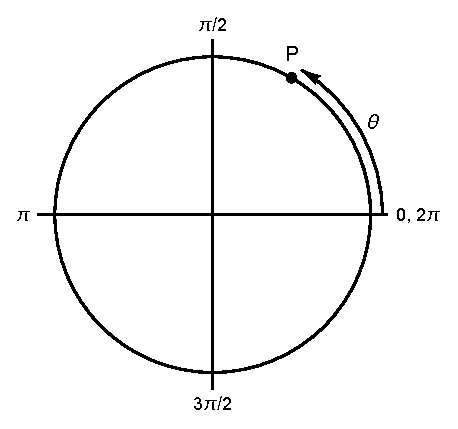
\includegraphics[width=0.5\textwidth]{eps/prereqs/trigtldr.eps}
\end{figure}

The measure of angles by the length of the arc is in units called
\textit{radians}. Recall the circumference of a circle is $C=2\pi r$,
and so the circumference of a unit circle is $2\pi$. Thus $\pi$ represents
a $180^\circ$ angle. Some common angles in radians are
$2\pi, \pi,\frac{\pi}{2}, \frac{\pi}{3}, \frac{\pi}{4}, \frac{\pi}{6}$, and
$\frac{3\pi}{2}$. To convert these to degrees simply replace $\pi$ with
$180$, and compute the fraction.

\vs

It should be self-evident that adding $2\pi$ to an angle results in the
angle itself; and that adding $\frac{\pi}{2}$ to an angle shifts it by
$90^{\circ}$. Further:
\[(\cos 0,\sin 0)=(1,0)\ \ \ \ \ \text{and}\ \ \ \ \ (\cos \frac{\pi}{2},\sin \frac{\pi}{2})=(0,1)\]

\clearpage
\subsubsection*{Plotting}
It is not too difficult to plot trigonometric functions. Consider some
properties of cosine we've already seen (or can easily deduce):
$\cos 0=1$, $\cos \frac{\pi}{2}=0$, $\cos \pi=-1$. We've also seen that
$\cos{(x+2\pi)}=\cos x$. The $x$-axis below covers $[-3\pi, 3\pi]$ (i.e. a
total length of $6\pi$). Since cosine repeats every $2\pi$, we should
expect the graph to repeat thrice. And this is exactly what we see.
\begin{figure}[htbp]
  \centering
  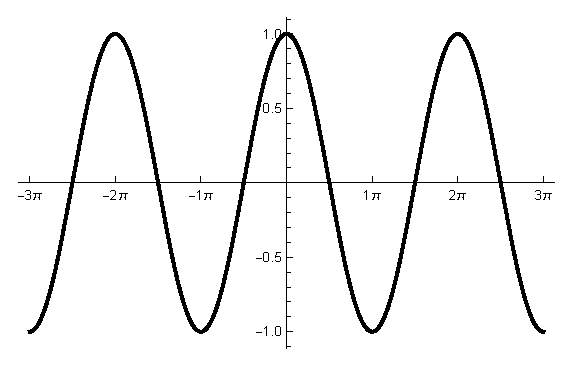
\includegraphics[width=.75\textwidth]{eps/prereqs/cosine.eps}
\end{figure}

We can easily increase the frequency by plotting $y=\cos cx$. Here we
double the frequency with $c=2$:
\begin{figure}[htbp]
  \centering
  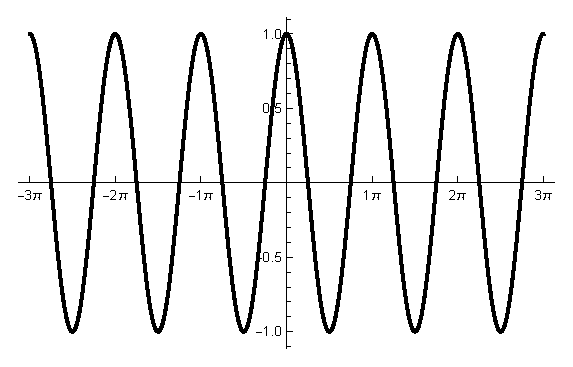
\includegraphics[width=.75\textwidth]{eps/prereqs/cosine2x.eps}
\end{figure}

\clearpage
\subsection{Limits}

\textbf{Claim 1a:} Let $f(x)=x\sin \frac{1}{x}$. Then
$\lim_{x\to0}f(x)=0$.

\textbf{Proof.} Let $\epsilon>0$ be given. We must show
$0<|x-0|<\delta$ implies $|f(x)-0|<\epsilon$. This is easy if you recall
the co-domain of $\sin$ is $[-1,1]$. This implies:
\[\left|x\sin \frac{1}{x}\right|\leq |x|\]

Thus fixing $|x|<\epsilon$ implies
$\left|x\sin \frac{1}{x}\right|<\epsilon$ as desired.



\vs---\vs

\textbf{Claim 1b:} Let $f(x)=x^2\sin \frac{1}{x}$. Then
$\lim_{x\to0}f(x)=0$.

\textbf{Proof.} By the same reasoning as above,
$\left|x^2\sin \frac{1}{x}\right|\leq x^2$. Thus fixing $|x|<\sqrt{\epsilon}$
implies $\left|x^2\sin \frac{1}{x}\right|<\epsilon$ as desired.

\vs---\vs

\textbf{Claim 1c:} Let $f(x)=\sqrt{|x|}\sin \frac{1}{x}$. Then
$\lim_{x\to0}f(x)=0$.

\textbf{Proof.} By the same reasoning as above,
$\left|\sqrt{|x|}\sin \frac{1}{x}\right|\leq \sqrt{|x|}$. Thus fixing
$|x|<\epsilon^2$ implies
$\left|\sqrt{|x|}\sin \frac{1}{x}\right|\leq \epsilon$ as desired.


\vs---\vs

\textbf{Claim 2:} $\lim_{x\to0}\sin \frac{1}{x}$ does not exist.

\textbf{Proof.}

\vs---\vs

\textbf{Claim 3:} $\lim_{x\to\infty}\sin \frac{1}{x}=0$.

\textbf{Proof.}

\subsection{Continuity}

\textbf{Claim 1:} $f(x)=\sin \frac{1}{x}$, $g(x)=x\sin \frac{1}{x}$ are not continuous at $0$.

\textbf{Proof.}

\vs---\vs

\textbf{Claim 2:} Let
\[G(x)=\begin{cases}
  x\sin \frac{1}{x},&x\neq0\\
  0,&x=0
\end{cases}\]
Then $G$ is continuous at $0$.

\vs

\textbf{Proof.}

\vs---\vs

\textbf{Claim 3:} Let
\[F(x)=\begin{cases}
  \sin \frac{1}{x},&x\neq0\\
  a,&x=0
\end{cases}\]
Then $F$ is \textit{not} continuous at $0$, for any choice of $a$.

\vs

\textbf{Proof.}

\vs---\vs

\textbf{Claim 4:} Let
\[f(x)=\begin{cases}
  x\sin \frac{1}{x},&x\neq0\\
  0,&x=0
\end{cases}\]
Then $f$ is continuous at $a$ for $a\neq 0$.

\vs

\textbf{Proof.}


\subsection{Derivatives}

\textbf{Claim 1:} Let
\[f(x)=\begin{cases}
  x\sin \frac{1}{x},&x\neq0\\
  0,&x=0
\end{cases}\]
Then $f$ is not differentiable at $0$.

\vs

\textbf{Proof.}

\vs---\vs

\textbf{Claim 2:} Let
\[g(x)=\begin{cases}
  x^2\sin \frac{1}{x},&x\neq0\\
  0,&x=0
\end{cases}\]
Then $g$ is differentiable at $0$.

\vs

\textbf{Proof.}

\subsection{Differentiation}

\textbf{Claim 1:} $g'$ is not differentiable at $0$.

\textbf{Proof.}

\vs---\vs

\textbf{Claim 2:} Let
\[f(x)=\begin{cases}
  x^3\sin \frac{1}{x},&x\neq0\\
  0,&x=0
\end{cases}\]
Then $f'$ is not differentiable at $0$.

\vs

\textbf{Proof.}

\vs---\vs

\textbf{Claim 3:} Let
\[f(x)=\begin{cases}
  x^4\sin \frac{1}{x},&x\neq0\\
  0,&x=0
\end{cases}\]
Then $f''$ is not differentiable at $0$.

\vs

\textbf{Proof.}

\vs

\textbf{TODO more stuff on pp 178}

%%% Local Variables:
%%% TeX-master: "notes"
%%% End:

\clearpage

\section{Derivatives, Part II (Differentiation)}

\subsection{Basic proofs}

We now prove theorems that make differentiation of a large class of
functions easy.

\vs

\textbf{Theorem 1.} If $f(x)=c$ then $f'(a)=0$ for all $a$.

\vs

\textit{Intuitively} derivatives measure the rate of change. A
constant function doesn't change, thus the derivative is zero.

\vs

\textbf{Proof:} we already proved this in the previous chapter.

\vs---\vs

\textbf{Theorem 2.} If $f(x)=x$ then $f'(a)=1$ for all $a$.

\vs

\textit{Intuitively} $f(x)$ grows at exactly the same rate as $x$,
thus the derivative is $1$.

\vs

\textbf{Proof:}
\[f'(a)=\lim_{h\to0}\frac{f(a+h)-f(a)}{h}=\lim_{h\to0}\frac{a+h-a}{h}=1\]

\vs---\vs

\textbf{Theorem 3.} If $f,g$ are differentiable at $a$, then
$(f+g)'(a)=f'(a)+g'(a)$.

\vs
\textit{Examples:}
\begin{itemize}
\item You have two functions, each modeling growth of some bank
  account. You want to understand the rate of growth of both accounts.
\item You have two different assembly lines producing the same
  product. $c_1(x)$ and $c_2(x)$ model the cost of producing $x$
  units on each assembly line. You want to understand total cost
  changes as production across both assembly lines increases.
\end{itemize}

\textbf{Proof:}
\begin{align*}
  (f+g)'(a)&=\lim_{h\to0}\frac{(f+g)(a+h)-(f+g)(a)}{h}\\
           &=\lim_{h\to0}\frac{f(a+h)+g(a+h)-f(a)-g(a)}{h}\\
           &=\lim_{h\to0}\frac{f(a+h)-f(a)}{h} +
             \lim_{h\to0}\frac{g(a+h)-g(a)}{h}\\
           &=f'(a)+g'(a)
\end{align*}

---\vs

\textbf{Theorem 4.} If $f,g$ are differentiable at $a$, then
\[(f\cdot g)'(a)=f'(a)\cdot g(a)+f(a)\cdot g'(a)\]

\vs

\textit{Examples:}
\begin{itemize}
\item Let $r_1(t), r_2(t)$ model the length of each side of a
  rectangle over time. You want to understand the change in area at
  time $t$.
\end{itemize}

\textbf{Proof:}
\begin{align*}
(f\cdot g)'(a)=&=\lim_{h\to0}\frac{(f\cdot g)(a+h)-(f\cdot g)(a)}{h}\\
           &=\lim_{h\to0}\frac{f(a+h)g(a+h)-f(a)g(a)}{h}\\
           &=\lim_{h\to0}\frac{f(a+h)g(a+h)-f(a)g(a) + f(a+h)g(a)-f(a+h)g(a)}{h}\\
           &=\lim_{h\to0}\frac{f(a+h)(g(a+h)-g(a)) + g(a)(f(a+h) - f(a))}{h}\\
           &=\lim_{h\to0}\left(f(a+h)\frac{g(a+h)-g(a)}{h}+g(a)\frac{f(a+h)-f(a)}{h}\right)\\
           &=\lim_{h\to0}f(a+h)\cdot\lim_{h\to0}\frac{g(a+h)-g(a)}{h}+\lim_{h\to0}g(a)\cdot\lim_{h\to0}\frac{f(a+h)-f(a)}{h}\\
           &=\lim_{h\to0}f(a+h)\cdot g'(a)+g(a)\cdot f'(a)
\end{align*}
Recall from \ref{diff-implies-cont} that if $f$ is differentiable at
$a$, then $\lim_{h\to0}f(a+h)=f(a)$. Thus
\[(f\cdot g)'(a)=f(a)\cdot g'(a)+g(a)\cdot f'(a)\]

---\vs

\textbf{Theorem 5.} If $g(x)=cf(x)$ then $g'(a)=c\cdot f'(a)$.

\vs

\textit{Examples:}
\begin{itemize}
\item Let $h$ be a height of a rectangle that's constant, and let
  $b(t)$ model the length of the base of a rectangle over time. You
  want to understand the change in area at time $t$.
\end{itemize}

\textbf{Proof:} Let $h(x)=c$ so $g=h\cdot f$. Then by theorem 4:
\begin{align*}
  g'(x)&=h'(x)f(x)+f'(x)g(x)\\
       &=0\cdot f(x)+cf'(x)\\
       &=cf'(x)
\end{align*}

---\vs

\textbf{Theorem 6.} If $f(x)=x^n$ for $n\in\mathcal{N}$, then $f'(a)=na^{n-1}$ for
all $a$.

\vs

\textit{Examples:}
\begin{itemize}
\item Let $s(t)$ model the length of the side of a cube over time. You
  want to understand the change in volume at time $t$.
\end{itemize}

\textbf{Proof.} We prove this by induction. For $n=1$, $f'(a)=1$ by
theorem 2.

\vs

Assume if $f(x)=x^n$ then $f'(a)=na^{n-1}$ for all $a$.

\vs

Let $I(x)=x$ and let $g(x)=x^{n+1}=xx^n$. Then $g(x)=I(x)\cdot f(x)$, i.e.
$g=I\cdot f$. By theorem 4:
\begin{align*}
  g'(a)&=(I\cdot f)'(a)\\
       &=I'(a)f(a)+I(a)f'(a)\\
       &=1\cdot a^n+a\cdot na^{n-1}\\
       &=a^n+na^n\\
       &=a^n(1+n)\\
       &=(n+1)a^n
\end{align*}

---\vs

\textbf{Theorem 7.} If $g$ is differentiable at $a$ and $g(a)\neq0$, then
\[\left(\frac{1}{g}\right)'(a)=\frac{-g'(a)}{{[g(a)]}^2}\]

\textit{Examples:}
\begin{itemize}
\item Let $i(d)=\frac{1}{d^2}$ model the intensity of light, which
  is inversely proportional to the square of the distance from the
  source. You want to know how intensity changes with distance.
\end{itemize}

\textbf{Proof.} We will prove this by using the derivative definition.
However, we must first show $\left(\frac{1}{g}\right)(a+h)$ is defined
for sufficiently small $h$. This is easy.

\vs

Since $g$ is differentiable at $a$ it is continuous at $a$. Thus by
nonzero neighborhood lemma (see \ref{subsubsec:nonzero-lemma}) there
exists $\delta>0$ such that $|h|<\delta$ implies $g(a+h)\neq0$ for all
$h$. Thus $\left(\frac{1}{g}\right)(a+h)$ is defined for sufficiently
small $h$.

\vs

We are now ready to prove the core of the theorem.
\begin{align*}
  \lim_{h\to0}\frac{\left(\frac{1}{g}\right)(a+h)-\left(\frac{1}{g}\right)(a)}{h}
  &=\lim_{h\to0}\left(\frac{1}{g(a+h)}-\frac{1}{g(a)}\right)/h\\
  &=\lim_{h\to0}\left(\frac{g(a)-g(a+h)}{g(a)\cdot g(a+h)}\right)/h\\
  &=\lim_{h\to0}\frac{g(a)-g(a+h)}{h\cdot g(a)\cdot g(a+h)}\\
  &=\lim_{h\to0}\frac{-[g(a+h)-g(a)]}{h}\cdot\frac{1}{g(a)\cdot g(a+h)}\\
  &=\lim_{h\to0}\frac{-[g(a+h)-g(a)]}{h}\cdot\lim_{h\to0}\frac{1}{g(a)\cdot
    g(a+h)}
\end{align*}

Recall from \ref{diff-implies-cont} that if $f$ is differentiable at
$a$, then $\lim_{h\to0}f(a+h)=f(a)$. Thus:
\begin{align*}
  \lim_{h\to0}\frac{-[g(a+h)-g(a)]}{h}\cdot\lim_{h\to0}\frac{1}{g(a)\cdot g(a+h)}
  &=-g'(a)\cdot \frac{1}{[g(a)]^2}
\end{align*}

as desired.

\vs---\vs

\textbf{Theorem 8.} If $f, g$ are differentiable at $a$ and $g(a)\neq0$, then
\[\left(\frac{f}{g}\right)'(a)=\frac{g(a)\cdot f'(a)-f(a)\cdot g'(a)}{[g(a)]^2}\]

\vs

\textit{Examples:}
\begin{itemize}
\item Let $e(t), s(t)$ model the number of engineers and sales people
  at a company over time. You want to understand the change in the
  ratio between the two.
\end{itemize}

\textbf{Proof.}
\begin{align*}
  \left(\frac{f}{g}\right)'(a)&=\left(f\cdot\frac{1}{g}\right)'(a)\\
  &=f(a)\cdot
    \left(\frac{1}{g}\right)'(a)+f'(a)\cdot\left(\frac{1}{g}\right)(a)\\
  &=\frac{-g'(a)\cdot f(a)}{[g(a)]^2}+\frac{f'(a)}{g(a)}\\
  &=\frac{-g'(a)\cdot f(a)\cdot g(a)+f'(a)\cdot [g(a)]^2}{[g(a)]^3}\\
  &=\frac{f'(a)\cdot g(a)-g'(a)\cdot f(a)}{[g(a)]^2}\\
\end{align*}

\subsection{Chain rule}
The derivative of composed functions is considerably more complicated,
and so deserves its own section. We'll prove this in two stages.
First, we'll attempt a proof with a few false starts that will point
us in the direction of a real proof. Once the direction becomes clear,
we'll abandon our first draft and write a clean proof from scratch.

\vs

\textbf{Theorem 9 (the chain rule).} If $g$ is differentiable at $a$,
and $f$ is differentiable at $g(a)$, then
\[(f\circ g)'(a)=f'(g(a))\cdot g'(a)\]

\textit{Examples:}
\begin{itemize}
\item Let $a(t)$ model altitude of a rocket over time, and let $p(a)$
  model air pressure at a particular altitude. You want to know how
  air pressure changes over time.
\end{itemize}

\subsubsection*{Proof, first draft.}

As usual, we start with the definition of the derivative:
\begin{align*}
  (f\circ g)'(a)&=\lim_{h\to0}\frac{(f\circ g)(a+h)-(f\circ g)(a)}{h}\\
            &=\lim_{h\to0}\frac{f(g(a+h))-f(g(a))}{h}\\
            &=\lim_{h\to0}\left(\frac{f(g(a+h))-f(g(a))}{g(a+h)-g(a)}\cdot\frac{g(a+h)-g(a)}{h}\right)\\
            &=\lim_{h\to0}\frac{f(g(a+h))-f(g(a))}{g(a+h)-g(a)}\cdot\lim_{h\to0}\frac{g(a+h)-g(a)}{h}\\
            &=\left(\lim_{h\to0}\frac{f(g(a+h))-f(g(a))}{g(a+h)-g(a)}\right)\cdot g'(a)
\end{align*}

This is a bit of a false start as we now have two problems:
\begin{itemize}
\item To get $f'(g(a))$ in the first term, we need
  $\lim_{h\to0}\frac{f(g(a)+h)-f(g(a))}{h}$, but instead we have
  $\lim_{h\to0}\frac{f(g(a+h))-f(g(a))}{g(a+h)-g(a)}$.
\item $g(a+h)-g(a)$ may be zero for $h\neq 0$, so the division may be
  illegal.
\end{itemize}

However it isn't a total waste. Our false start gives us an idea for
how we may proceed-- we'll replace
$\frac{f(g(a+h))-f(g(a))}{g(a+h)-g(a)}$ with something
better. What could be the replacement? Let's hypothesize existance of
a function $\phi(h)$ with the following property (we will soon prove such
a function exists):

\[\frac{f(g(a+h))-f(g(a))}{h}=\phi(h)\cdot\frac{g(a+h)-g(a)}{h}\]

We can then rewrite our initial equations as follows:
\begin{align*}
  (f\circ g)'(a)&=\lim_{h\to0}\frac{(f\circ g)(a+h)-(f\circ g)(a)}{h}\\
            &=\lim_{h\to0}\frac{f(g(a+h))-f(g(a))}{h}\\
            &=\lim_{h\to0}\left(\phi(h)\cdot\frac{g(a+h)-g(a)}{h}\right)\\
            &=\lim_{h\to0}\phi(h)\cdot\lim_{h\to0}\frac{g(a+h)-g(a)}{h}\\
            &=\lim_{h\to0}\phi(h)\cdot g'(a)
\end{align*}

To get to $(f\circ g)'(a)=f'(g(a))\cdot g'(a)$ we need $\phi(h)$ to possess one
more property:
\[\lim_{h\to0}\phi(h)=f'(g(a))\]

Given this additional property, we can now finish our reasoning:
\[(f\circ g)'(a)=\lim_{h\to0}\phi(h)\cdot g'(a)=f'(g(a))\cdot g'(a)\]

Thus proving the chain rule reduces to proving there exists a function
$\phi(h)$ with the two properties above. For cleanliness, let's start a
new proof from scratch and demonstrate the existance of such a
function.

\subsubsection*{Proof.}

Suppose there exists a function $\phi(h)$ with the
following properties:
\setcounter{equation}{0}
\begin{gather}
\frac{f(g(a+h))-f(g(a))}{h}=\phi(h)\cdot\frac{g(a+h)-g(a)}{h}\\
\lim_{h\to0}\phi(h)=f'(g(a))
\end{gather}

Then
\begin{align*}
  (f\circ g)'(a)&=\lim_{h\to0}\frac{(f\circ g)(a+h)-(f\circ g)(a)}{h}\\
            &=\lim_{h\to0}\frac{f(g(a+h))-f(g(a))}{h}\\
            &=\lim_{h\to0}\left(\phi(h)\cdot\frac{g(a+h)-g(a)}{h}\right)&\text{by
                                                                 property
                                                                 1}\\
            &=\lim_{h\to0}\phi(h)\cdot\lim_{h\to0}\frac{g(a+h)-g(a)}{h}\\
            &=\lim_{h\to0}f'(g(a))\cdot g'(a)&\text{by property 2}
\end{align*}

To complete the proof we must construct such a function and prove our
construction has properties 1 and 2. We will do so now. Define $\phi$ as
follows:
\begin{align*}
  \phi(h)=\begin{cases}
    \frac{f(g(a+h))-f(g(a))}{g(a+h)-g(a)} & \text{if } g(a+h)-g(a)\neq0 \\
    f'(g(a))  & \text{if } g(a+h)-g(a)=0
\end{cases}
\end{align*}

We will prove properties 1 and 2 hold for $\phi$.

\vs

\textbf{Property 1 proof.}

We now show
$\frac{f(g(a+h))-f(g(a))}{h}=\phi(h)\cdot\frac{g(a+h)-g(a)}{h}$. There are
two cases: either $g(a+h)-g(a)\neq0$ or $g(a+h)-g(a)=0$. Suppose
$g(a+h)-g(a)\neq0$. Then
\begin{align*}
  \phi(h)\cdot\frac{g(a+h)-g(a)}{h}&=\frac{f(g(a+h))-f(g(a))}{g(a+h)-g(a)}\cdot\frac{g(a+h)-g(a)}{h}\\
                            &=\frac{f(g(a+h))-f(g(a))}{h}
\end{align*}

Alternatively, suppose $g(a+h)-g(a)=0$. Then
\begin{align*}
  \phi(h)\cdot\frac{g(a+h)-g(a)}{h}&=f'(g(a))\cdot\frac{g(a+h)-g(a)}{h}\\
                            &=f'(g(a))\cdot\frac{0}{h}\\
                            &=0
\end{align*}

But $g(a+h)-g(a)=0$ means $g(a+h)=g(a)$, and thus
$\frac{f(g(a+h))-f(g(a))}{h}=0$. Thus in both cases property 1 holds,
as desired.

\vs

\textbf{Property 2 proof.}

We now show $\lim_{h\to0}\phi(h)=f'(g(a))$. Put differently:
\begin{itemize}
\item \textit{Intuitively}, we're trying to show that when $h$ is
  small, the top piece of $\phi$ piecewise definition approaches the
  bottom piece (which we chose to be $f'(g(a))$).
\item Here is another way to frame it. Observe that
  $\phi(0)=f'(g(a))$. Thus showing $\lim_{h\to0}\phi(h)=f'(g(a))$ is
  equivalent to showing $\lim_{h\to0}\phi(h)=\phi(0)$, i.e. that
  $\phi$ is continuous at $0$.
\item Formally, we must show that given $\epsilon>0$ there exists
  $\delta>0$ such that $|h|<\delta$ implies $|\phi(h)-f'(g(a))|<\epsilon$.
\end{itemize}

So, let $\epsilon>0$ be given.

\vs

\textit{Firstly}, since $f$ is differentiable at $g(a)$, by definition
of the derivative we have:
\[f'(g(a))=\lim_{k\to0}\frac{f(g(a)+k)-f(g(a))}{k}\]

Inlining the limit defition, for all $\epsilon>0$ there exists
$\delta'>0$ such that $0<|k|<\delta'$ implies
\[\left|\frac{f(g(a)+k)-f(g(a))}{k}-f'(g(a))\right|<\epsilon\]

\textit{Secondly}, since $g$ is differentiable at $a$, it continuous
at $a$. Thus:
\[\lim_{h\to0}g(a+h)=g(a)\]

Or put differently, there exists $\delta>0$ such that $|h|<\delta$ implies:
\[|g(a+h)-g(a)|<\delta'\]

\textit{Finally}, we now have everything we need to prove property 2.
Consider any $h$ with $|h|<\delta$.
\begin{itemize}
\item If $g(a+h)-g(a)=0$ then $\phi(h)=f'(g(a))$ so $|\phi(h)-f'(g(a))|<\epsilon$.
\item If $g(a+h)-g(a)\neq0$ we can fix $k=g(a+h)-g(a)$ as both aren't
  $0$ and are less than $\delta'$. Thus we get:
\begin{align*}
  \epsilon&>\left|\frac{f(g(a)+k)-f(g(a))}{g(a+h)-g(a)}-f'(g(a))\right|\\
  &=\left|\frac{f(g(a)+g(a+h)-g(a))-f(g(a))}{g(a+h)-g(a)}-f'(g(a))\right|\\
  &=\left|\frac{f(g(a+h))-f(g(a))}{g(a+h)-g(a)}-f'(g(a))\right|\\
  &=\left|\phi(h)-f'(g(a))\right|
\end{align*}
I.e. $\left|\phi(h)-f'(g(a))\right|<\epsilon$ as desired.
\end{itemize}



\subsection{Implications}
Theorems 1-5 imply:
\[(-f)'(a)=(-1\cdot f')(a)=-f'(a)\]
\begin{center}and\end{center}
\[(f-g)'(a)=(f+(-g))'(a)=f'(a)+(-g)'(a)=f'(a)-g'(a)\]

\subsection{Trig}

%%% Local Variables:
%%% TeX-master: "notes"
%%% End:

\clearpage

\section{Derivatives, Part III (Consequences)}

This chapter builds up to two new capabilities. The first is graph
sketching (or put differently, using features of the derivative to
approximate shapes of functions). The second is L'H\^opital's rule,
which allows us to take limits of the form $\frac{0}{0}$. We build up
to these capabilities by studying the consequences of the derivative.
On the way we prove the Mean Value Theorem, one of key calculus
results.

\vs

I reordered content from Spivak's chapter for clarity, but kept the
theorem and corollary numbering scheme. Thus theorem numbers here
aren't in order, but they match the numbers in Spivak.\footnote{This
  was the most meandering of Spivak's chapters; it took \textit{a lot}
  of reordering for the overall structure to make sense. Not sure if
  it's the material, the presentation, or just me losing steam, but
  getting through this chapter took forever. By the end of it I was
  bored to tears, barely able to force myself to finish it.}

\subsection{Maxima and manima}
We start with some definitions. Let $f$ be a function and $A$ a set of
numbers contained in $f$'s domain.\footnote{$A$ need not have any
  additional properties. E.g. it may have holes, etc.} Then:

\vs

\textbf{Definition.} A point $x$ in $A$ is a \textbf{maximum
  point} for $f$ on $A$ if
\[f(x)\geq f(y)\qquad\text{for every $y$ in $A$}\]

\textbf{Definition.} A \textbf{critical point} of $f$ is a number $x$
such that $f'(x)=0$.\footnote{If $x$ is a maximum and/or critical
  point, then $f(x)$ is called a maximum and/or critical value of
  $f$.}

\vs---\vs

\textbf{Theorem 1a.} Let $f$ be any function defined on $(a,b)$. If $x$
is a maximum point for $f$ on $(a,b)$, and $f$ is differentiable at
$x$, then $f'(x)=0$.

\vs

\textit{Intuitively,} maximum and minimum points are also critical
points (but \textbf{not} the other way around-- $f(x)=x^3$ has
$f'(0)=0$ as an obvious counterexample\footnote{In this case this
  critical point is called the \textbf{saddle point}.}).

\vs

\textbf{Proof.} \textit{Informally}, suppose $a$ is a maximum point.
Draw a secant line between $a$ and $a_l$ (to its left), and another
line between $a$ and $a_r$ (to its right). The $a-a_l$ line will slope
up, the $a-a_r$ line will slope down. Thus at $a$ the slope crosses
from positive to negative, and is $0$.

\vs

\textit{Formally}, let $h\in\mathcal{R}$ such that $x+h\in(a,b)$. If $h<0$ it follows that:
\begin{align*}
  &f(x+h)\leq f(x)&\text{since $f(x)$ is a maximum value}\\
  &\implies f(x+h)-f(x)\leq 0\\
  &\implies\frac{f(x+h)-f(x)}{h}\geq0&\text{dividing by negative $h$}\\
  &\implies \lim_{h\to0^-}\frac{f(x+h)-f(x)}{h}\geq0&\text{see
                                                 \ref{subsec:onesided-limits}
                                                 and
                                                 \ref{subsubsec:nonzero-lemma}}
\end{align*}

Conversely, if $h>0$ it follows that:
\begin{align*}
  &\implies \frac{f(x+h)-f(x)}{h}\leq0&\text{dividing by positive $h$}\\
  &\implies \lim_{h\to0^+}\frac{f(x+h)-f(x)}{h}\leq0
\end{align*}

By hypothesis, $f$ is differentiable at $x$. Thus the two limits must
be equal to each other, and to $f'(x)$. Therefore $f'(x)\geq0$ and
$f'(x)\leq0$. Thus $f'(x)=0$ as desired.

\vs

\textbf{Theorem 1b.} Let $f$ be any function defined on $(a,b)$. If
$x$ is a \textit{minimum} point for $f$ on $(a,b)$, and $f$ is
differentiable at $x$, then $f'(x)=0$.

\vs

\textbf{Proof.} Let $g=-f$. Then $x$ is a maximum point of $g$. By 1a,
$g'(x)=0$, thus $(-f)'(x)=-1\cdot f'(x)=0$, and thus $f'(x)=0$ as desired.

\vs---\vs

The obvious (extremely valuable) consequences of these theorems is
that we can find minimum and maximum values of $f$ by solving for
$f'(x)=0$.

\subsubsection*{On closed intervals}
If $x$ is a maximum or minimum point for $f$ on $[a,b]$, then $x$ must
be in one of three classes:
\begin{enumerate}
\item The critical points of $f$ in $[a,b]$.
\item The end points $a$ and $b$.
\item Points $x\in[a,b]$ such that $f$ is not differentiable at $x$.
\end{enumerate}

(If $x$ is not in second or third group, then $x\in(a,b)$ and $f'(x)$
exists; thus $f'(x)=0$ by Theorem 1, and thus $x$ is in the first
group.)

\subsubsection*{On open intervals}

On open intervals we don't necessarily know minimum or maximum values
exist, so these problems require creative work. For example, recall we
showed even degree polynomials have a minimum value (see
\ref{even-poly-root}). Now that we've done that work for even $n$ and
$f(x)=x^{n}+a_{n-1}x^{n-1}+\ldots+a_{0}$, we can solve for $x$ in
$f'(x)=0$ to find minimal values. But because the interval is open, we
had to do the work in \ref{even-poly-root} to show minimal value
exists first.

\subsection{Mean Value Theorem}

\textbf{Theorem 3 (Rolle's theorem).} Let $f$ be continuous on $[a,b]$
differentiable on $(a,b)$, and let $f(a)=f(b)$. Then there exists
$x\in(a,b)$ such that $f'(x)=0$.

\vs

\textbf{Proof.} There are two cases:
\begin{itemize}
\item \textit{Case 1.} Suppose the maximum or the minimum occurs at a
  point $x\in(a,b)$. Then $f'(x)=0$ by theorem 1, and we are done.
\item \textit{Case 2.} Suppose the maximum and the minimum both occur
  at endpoints. Since $f(a)=f(b)$, the maximum and the minimum values
  are equal and $f$ is constant. Then for any $x\in(a,b), f'(x)=0$ and
  we are done.
\end{itemize}

\vs---\vs

\textbf{Claim:} Let $f(x)=a_nx^n+a_{n-1}x^{n-1}+\ldots+a_0$. Then
$f$ has at most $n$ roots.

\vs

\textbf{Proof.}\footnote{This is normally an algebraic theorem, but in
  the interest of pedagogy Caclulus offers an easy proof.} Suppose
$x_1, x_2$ are roots of $f$, i.e. $f(x_1)=f(x_2)=0$. Then by Rolle's
theorem there exists $x_1<x<x_2$ such that $f'(x)=0$. Thus if $f$ has
$k$ different roots $x_1<x_2<\ldots<x_k$, it follows $f'$ has at least
$k-1$ different roots (one between $x_1$ and $x_2$, one between $x_2$
and $x_3$, etc.)

\vs

It is now easy to prove our claim by induction. It's easy to see
\[f(x)=a_nx^n+a_{n-1}x^{n-1}+\ldots+a_0\]

has at most one root for $n=1$. Assume the claim is true for $n$.
Consider the polynomial
\[g(x)=b_{n+1}x^{n+1}+b_nx^n+\ldots+b_0\] Suppose for contradiction
$g$ has \textit{more} than $n+1$ roots. Then by the argument in the
first paragraph, $g'$ would have more than $n$ roots. But we assumed
the claim holds for $n$, a contradiction. Thus $g$ has at most $n+1$
roots as desired.


\vs---\vs

\textbf{Claim:} Let $f(x)=a_nx^n+a_{n-1}x^{n-1}+\ldots+a_0$. Then
$f$ has at most $n-1$ critical points.

\vs

\textbf{Proof.} This is easy. Observe that
\[f'(x)=a_n n x^{n-1} + a_{n-1} (n-1) x^{n-2} + \dots + a_1\] Thus by
previous claim, $f'$ has at most $n-1$ roots, and thus at most $n-1$
critical points.

\vs---\vs

\textbf{Theorem 4 (Mean value theorem).}

Let $f$ be continuous on $[a,b]$ and differentiable on $(a,b)$. Then
there exists $x\in(a,b)$ such that:
\[f'(x)=\frac{f(b)-f(a)}{b-a}\]

Here are three intuitions:
\begin{enumerate}
\item \textit{Geometric intuition.} There exists a line tangent to $f$
  parallel to the line between the endpoints (i.e. line between
  $(a, f(a))$ and $(b, f(b))$).
\item \textit{Algebraic intuition.} There exists a point $x$ at which
  instantaneous rate of change of $f$ is equal to the average change
  of $f$ on $[a,b]$.
\item \textit{Physical example.} If you travel 60 miles in one hour,
  at some point you must have been travelling exactly 60 miles per
  hour.
\end{enumerate}

\textbf{Proof.}

Here's an informal proof outline:
\begin{itemize}
\item Take the line segment formed by endpoints $(a,f(a))$ and
  $(b,f(b))$.
\item Construct a function $g$ that for $x\in(a,b)$ returns the vertical
  distance between $f(x)$ and the line segment. (We'll show it's
  continuous and differentiable.)\footnote{It turns out not to matter
    whether $g$ computes the distance between $f$ and the line
    segment, or $f$ and the line segment shifted down by $f(a)$ (i.e.
    down to $x$-axis). So in practice we use the lattern form to avoid
    dealing with the $f(a)$ term in the linear equation.}
\item By Rolle's theorem, it has a flat tangent. It's easy to show
  algebraically (and visualize geometrically) this proves the MVT.
\end{itemize}

Formally, let\footnote{See \ref{subsubsec-point-slope-form} for how
  the point-slope form is used to construct the second term.}
\[h(x)=f(x)-\left[\frac{f(b)-f(a)}{b-a}(x-a)\right]\]

Observe $h$ is continuous on $[a,b]$ and differentiable on $(a,b)$.
Further:
\begin{align*}
  h(a)&=f(a)-\left[\frac{f(b)-f(a)}{b-a}\cdot0\right]=f(a)\\
  h(b)&=f(b)-\left[\frac{f(b)-f(a)}{b-a}(b-a)\right]\\
      &=f(b)-[f(b)-f(a)]\\
      &=f(a)
\end{align*}

Thus we can apply Rolle's Theorem $h$ to conclude there is $x\in(a,b)$
such that:\footnote{Note the derivative of a line is its slope, thus
  $\frac{d}{dx}\left[\frac{f(b)-f(a)}{b-a}(x-a)\right]=\frac{f(b)-f(a)}{b-a}$.}

\begin{align*}
  &0=h'(x)=f'(x)-\frac{f(b)-f(a)}{b-a}\\
  &\implies f'(x)=\frac{f(b)-f(a)}{b-a}
\end{align*}

QED.

\vs---\vs

\textbf{MVT Corollary 1.} If $f$ is defined on an interval and $f'(x)=0$
for all $x$ in the interval, then $f$ is constant on the interval.

\vs

\textit{Intuitively,} if the velocity of a particle is always zero,
the particle must be standing still.

\vs

\textbf{Proof.} Let $a\neq b$ be any two points on the interval. Then
there is $x\in(a,b)$ such that $f'(x)=\frac{f(b)-f(a)}{b-a}$. But
$f'(x)=0$ for all $x$ on the interval, thus $0=\frac{f(b)-f(a)}{b-a}$.
Thuf $f(a)=f(b)$ for any $a,b$ (i.e. $f$ is constant on the interval
as desired).

\vs---\vs

\textbf{MVT Corollary 2.} If $f,g$ are defined on the same interval, and
$f'(x)=g'(x)$ for all $x$ in the interval, then there is
$c\in\mathcal{R}$ such that $f=g+c$.

\vs

\textbf{Proof.} Observe that
\begin{align*}
  &f'(x)=g'(x)\\
  &\implies f'(x)-g'(x)=0\\
  &(f-g)'(x)=0
\end{align*}

By corollary 1, $(f-g)$ is constant, i.e. $f=g+c$ as desired.

\subsection{Increasing and decreasing functions}

\textbf{Definition.} A function is \textbf{increasing} on an interval
if $f(a)<f(b)$ whenever $a,b$ are two numbers in the interval with
$a<b$.\footnote{The decreasing function definition is obvious.}

\vs

\textbf{MVT Corollary 3a.} If $f'(x)>0$ for all $x$ on an interval, then
$f$ is increasing on the interval.

\vs

\textbf{Proof.} Let $a<b$ be two points on an interval. Then there
exists $x\in(a,b)$ such that
\[f'(x)=\frac{f(b)-f(a)}{b-a}\]

But $f'(x)>0$ for all $x\in(a,b)$, thus
\[\frac{f(b)-f(a)}{b-a}>0\]

We know $b-a>0$, thus $f(b)>f(a)$ as desired.

\vs---\vs

\textbf{MVT Corollary 3b.} If $f'(x)<0$ for all $x$ on an interval, then
$f$ is decreasing on the interval.

\vs

\textbf{Proof.} The proof is an obvious modification of 3a.

\subsection{Local maxima and manima}
\textbf{Definition.} A point $x$ in $A$ is a \textbf{local maximum
  point} for $f$ on $A$ if there is some $\delta>0$ such that $x$ is a
maximum point for $f$ on $A\cap(x-\delta, x+\delta)$.

\vs

\textbf{Theorem 2.} If $f$ is defined on $(a,b)$ and has a local
maximum (or minimum) at $x$, and $f$ is differentiable at $x$, then
$f'(x)=0$.

\vs

\textbf{Proof.} The proof is a trivial application of theorem 1 to $f$
on $(x-\delta, x+\delta)$.

\vs---\vs

The opposite of theorem 2 isn't true-- if $f'(x)=0$ it does not
necessarily imply there is a local minimum or maximum at $x$ (consider
$f(x)=x^3$ at $x=0$ for example). Thus if we want to determine if a
point is a local maximum, we cannot use theorem 2 to make that
determination. We need some other way. The derivative offers us two
such tests to choose between.

\subsubsection*{First derivative test}

Suppose $f'(x)=0$. Check the sign of $f'$ on some interval to the
left and right of $x$. Then:
\begin{itemize}
\item If $f'>0$ to the left of $x$ and $f'<0$ to the right, then $x$
  is a local maximum (since $f$ is increasing to the left and
  decreasing to the right of $x$).
\item If $f'<0$ to the left of $x$ and $f'>0$ to the right, then $x$
  is a local minimum (since $f$ is decreasing to the left and
  increasing to the right of $x$).
\item Otherwise $x$ is a saddle point.
\end{itemize}

\subsubsection*{Second derivative test}

\textbf{Theorem 5.} Suppose $f'(a)=0$. If $f''(a)>0$, then $f$ has a
local minimum at $a$; if $f''(a)<0$, then $f$ has a local maximum at
$a$.

\vs

\textit{Intuitively,} $f''(a)>0$ means the slope of $f$ (represented
by $f'$) is increasing around $a$. Thus the curve must be sloping
upward.

\vs

\textbf{Proof.}
\begin{align*}
  f''(a)&=\lim_{h\to0}\frac{f'(a+h)-f'(a)}{h}&&\text{by derivative definition}\\
        &=\lim_{h\to0}\frac{f'(a+h)}{h}&&\text{$f'(a)=0$ by hypothesis}\\
\end{align*}

Suppose $f''(a)>0$. By nonzero neighborhood lemma (see
\ref{subsubsec:nonzero-lemma}), $f'(a+h)/h>0$ for sufficiently small
$h$. Therefore, for sufficiently small $h$:
\begin{itemize}
\item $f'(a+h)>0$ when $h>0$
\item $f'(a+h)<0$ when $h<0$
\end{itemize}

Thus by Corollary 3 of MVT:
\begin{itemize}
\item $f$ is increasing in some interval to the right of $a$
\item $f$ is decreasing in some interval to the left of $a$
\end{itemize}

Thus $f$ has a local minimum at $a$, as desired\footnote{The proof for
  $f''(a)<0$ is similar.}

\vs

(Note that theorem 5 gives no information if $f''(a)=0$.)

\vs---\vs

\textbf{Theorem 6.} Suppose $f''(a)$ exists. If $f$ has a local
minimum at $a$, then $f''(a)\geq0$; if $f$ has a local maximum at $a$,
then $f''(a)\leq 0$.

\vs

\textit{Intuitively,} this is a partial converse of thereom 5.

\vs

\textbf{Proof.} Suppose $f$ has a local minimum at $a$. Suppose for
contradiction $f''(a)<0$. Then by theorem 5 $f$ also has a local
maximum at $a$. Thefore $f$ is constant in some interval around $a$,
and so $f''(a)=0$. We have a contradiction, thus $f(a)\geq 0$, as
desired.\footnote{The proof for $f''(a)>0$ is similar.}


\subsection{Graph sketching}
We've now developed all the tools to get our first capability-- using
derivatives to approximate the shapes of graphs. Putting everything
together, to sketch a graph of a ``reasonable'' function $f$, follow
the following steps.

\vs

First of all, check if the function is even, or is odd.\footnote{Even
  functions are of the form $f(-x)=f(x)$ (i.e. symmetric about the
  $y$-axis). Odd functions are of the form $f(-x)=-f(x)$ (i.e.
  symmetric about the origin).} Symmetries can save a lot of time!
Then:

\begin{enumerate}
\item Express the domain of $f$ as a union of intervals.
\item Find limits as $f$ approaches \textit{open}
  endpoints.\footnote{Usually via one-sided and infinite limits, and
    limits at infinity.}
\item Find $f'$. Identify critical points (where $f'(x)=0$),
intervals where $f'>0$ (so $f$ is increasing), and intervals where
$f'<0$ (so $f$ is decreasing).
\item Use the first derivative test to identify local minima and
  maxima.
\item Plot obvious points (intercepts of axes, local minima and
  maxima, and points where the derivative doesn't exist). Interpolate
  the graph between them!
\end{enumerate}

\subsubsection*{Example 1}
First example is $f(x)=x^3+3x^2-9x+12$.

\begin{enumerate}
\item
\item 
\item 
\item 
\item 
\end{enumerate}

\subsubsection*{Example 2}
Second example is $f(x)=\frac{x^2}{1-x^2}$.

\begin{enumerate}
\item
\item 
\item 
\item 
\item 
\end{enumerate}

\subsection{L'H\^opital's rule}
We will build up to L'H\^opital's rule in the following way:

\begin{enumerate}
\item First, we'll cover a special case of L'H\^opital's rule (theorem
  7, no holes in derivatives).
\item To prove the L'H\^opital's rule we'll need Cauchy's Mean Value
  Theorem (a generalization of the Mean Value Theorem). When stated
  outright it can be hard to parse, so we'll build up to it informally
  next.
\item Formally prove Cauchy's Mean Value Theorem.
\item Prove L'H\^opital's rule.
\item We then reprove theorem 7 in a simpler way using L'H\^opital's
  rule.
\end{enumerate}

---\vs

\textbf{Theorem 7.} Suppose (1) $f$ is continuous at $a$, (2) $f'(x)$
exists for all $x$ in $0<|x-a|<\delta$, and (3) $\lim_{x\to a}f'(x)$ exists.
Then $f'(a)$ exists and
\[f'(a)=\lim_{x\to a}f'(x)\]

\textit{Intuitively,} derivatives cannot have holes. Put differently,
$f'$ \textit{can} be discontinuous at $a$ by fluctuating wildly near
$a$\footnote{In \ref{subsec-sine-poly} we've already seen an example
  of this:
  \[f(x)=\begin{cases}
    x^2\sin \frac{1}{x},&x\neq0\\
    0,&x=0.
  \end{cases}\]}, but
not by being undefined at $a$, or by being defined at $a$ to be far from its limit
near $a$.

\vs

\textbf{Proof 1.}\footnote{We will give a second proof in terms of
  L'H\^opital's rule at the end of this chapter.} Informally, for
``nice'' functions like $f$, the mean value theorem applies on tiny
scales of $\delta-\epsilon$ limits.

\vs

By derivative definition
\[f'(a)=\lim_{h\to 0}\frac{f(a+h)-f(a)}{h}\]

For sufficiently small $h$, both positive and negative, by supposition:
\begin{itemize}
\item $f$ will be continuous on $[a,a+h]$
\item $f$ will be differentiable on $(a,a+h)$
\end{itemize}

These conditions are sufficient for the mean value theorem, and thus
there exists $\alpha_h\in(a, a+h)$ such that:
\[\frac{f(a+h)-f(a)}{h}=f'(\alpha_h)\]

Putting this together:\footnote{Spivak observes the last equation in
  the proof is handwavy and needs a proper $\delta-\epsilon$ proof. I need to move
  on, so leaving this as a TODO.}
\begin{align*}
  f'(a)&=\lim_{h\to0}\frac{f(a+h)-f(a)}{h}&\text{by derivative definition}\\
       &=\lim_{h\to0}f'(\alpha_h)&\text{by mean value theorem}\\
       &=\lim_{x\to a}f'(x)&\text{$\alpha_h\in(a,a+h)$, thus as $h\to0$, $\alpha_h\to a$}
\end{align*}

\vs---\vs

\textbf{Theorem 8 (Cauchy's MVT), handwavy version.}

\vs

Let $f,g$ be continuous on $[a,b]$ and differentiable on $(a,b)$.
\textit{Intuitively,} theorem 8 states that there exists a point
$x\in(a,b)$ where $\frac{f'(x)}{g'(x)}$ (i.e. the ratio of
\textit{instantaneous} changes of $f$ and $g$) is the same as the
ratio of \textit{average} changes of $f$ and $g$ on $[a,b]$.

\vs

A more formal version of this is:
\begin{align*}
  \frac{f'(x)}{g'(x)}&=\frac{f(b)-f(a)}{b-a}\div \frac{g(b)-g(a)}{b-a}\\
                     &=\frac{f(b)-f(a)}{b-a}\cdot \frac{b-a}{g(b)-g(a)}\\
                     &=\frac{f(b)-f(a)}{g(b)-g(a)}
\end{align*}

when $g'(x)\neq 0$ and $g(b)-g(a)\neq0$.

\vs

There are two additional considerations. First, if $g(x)=x$ then
$g'(x)=1$, and the theorem simplifies to $f'(x)=\frac{f(b)-f(a)}{b-a}$
(i.e. we obtain the mean value theorem).

\vs

Second, to avoid division by zero constraints, formally the Cauchy
theorem is expressed as a multiplication rather than division of
terms:

\begin{align*}
  &\frac{f'(x)}{g'(x)}=\frac{f(b)-f(a)}{g(b)-g(a)}\\
  &\implies [f(b)-f(a)]g'(x)=[g(b)-g(a)]f'(x)
\end{align*}

With this buildup, we're ready to prove Cauchy's MVT.

\vs

\textbf{Theorem 8 (Cauchy's MVT).} Let $f,g$ be continuous on $[a,b]$
and differentiable on $(a,b)$. Then there exists $x\in(a,b)$ such that
\[[f(b)-f(a)]g'(x)=[g(b)-g(a)]f'(x)\]

\vs

\textbf{Proof.} Let
\[h(x)=f(x)[g(b)-g(a)]-g(x)[f(b)-f(a)]\]

Then $h$ is continuous on $[a,b]$ and differentiable on $(a,b)$.
Further observe that\footnote{If you plug $a$ and $b$ into $h(x)$, I
  promise this works (I checked).}
\[h(a)=f(a)g(b)-f(b)g(a)=h(b)\]

Thus $h(a)=h(b)$, Rolle's theorem applies, and there exists
$x\in(a,b)$ such that $h'(x)=0$. Taking the derivative of
$h$\footnote{Note to derive $h'$ we treat $g(b)-g(a)$ and $f(b)-f(a)$
  as constants.}:
\[0=h'(x)=f(x)'[g(b)-g(a)]-g(x)'[f(b)-f(a)]\]

---\vs

\textbf{Theorem 9 (L'H\^opital's rule.)} Suppose that
\[\lim_{x\to a}f(x)=0\qquad\text{and}\qquad\lim_{x\to a}g(x)=0\]

Then\footnote{Of course assuming $\lim_{x\to a}\frac{f'(x)}{g'(x)}$ exists.}
\[\lim_{x\to a}\frac{f(x)}{g(x)}=\lim_{x\to a}\frac{f'(x)}{g'(x)}\]

\textbf{Proof.} Recall Cauchy's MVT states that assuming $f,g$ are
continuous on $[a,b]$ and differentiable on $(a,b)$, there exists
$x\in(a,b)$ such that
\[\frac{f'(x)}{g'(x)}=\frac{f(b)-f(a)}{g(b)-g(a)}\]

\textit{Informally}, if we can make $f(a)=g(a)=0$, this equation will
start to look vaguely close to what we need. Assuming we can make it
work, we can then take limits of both sides to prove the L'H\^opital's
rule. This gives us a very rough outline of the proof.
\begin{enumerate}
\item For Cauchy's MVT to work we need to show continuity of $f$ and
  $g$.
\item ``Vaguely'' looking like what we need is not enough. We need to
  figure out how to map L'H\^opital's to Cauchy's MVT exactly.
\item To divide we need to show $g'(x)\neq0$ and $g(b)\neq0$.
\item Finally, we must take limits of both sides.
\end{enumerate}

We now proceed with formalizing each step.

\vs

\textit{Step 1:} Show $f,g$ are continuous.

\vs

By hypothesis $\lim_{x\to a}f(x)=0$ and $\lim_{x\to a}g(x)=0$. We don't
know the definitions of $f(a)$ and $g(a)$. But since in L'H\^opital's
rule we only care about limits, redefining $f(a)$ or $g(a)$ will not
affect the hypothesis. Thus, redefine $f(a)=g(a)=0$. Since now
$\lim_{x\to a}f(x)=f(a)$ and $\lim_{x\to a}g(x)=g(a)$, it follows
$f,g$ are now continuous.

\vs

\textit{Step 2:} Map L'H\^opital's rule to Cauchy's MVT.

\vs

Further by hypothesis, $\lim_{x\to a}f'(x)/g'(x)$ exists. By limit
definition $f'(x)$ and $g'(x)$ exist in the neighborhood of
$x\in(a-\delta, a+\delta)$ with the possible exception of $x=a$. Let's consider
all $x\in(a-\delta, a)$ and $x\in(a, a+\delta)$ separately.

\vs

For all $x\in(a-\delta, a)$ consider $f$ and $g$ on interval $[x,a]$. Both
are continuous on $[x,a]$ and differentiable on $(x,a)$, thus Cauchy's
MVT applies, i.e. there exists $\alpha\in(x,a)$ such that:
\begin{align*}
  &[f(a)-f(x)]g'(\alpha)=[g(a)-g(x)]f'(\alpha)\\
  &\implies -f(x)g'(\alpha)=-g(x)f'(\alpha)&&\text{since $f(a)=g(a)=0$}\\
  &\implies f(x)g'(\alpha)=g(x)f'(\alpha)&&\text{multiply both sides by $-1$}
\end{align*}

Similarly, for all $x\in(a, a+\delta)$ consider $f$ and $g$ on interval $[a,x]$. Both
are continuous on $[a,x]$ and differentiable on $(a,x)$, thus Cauchy's
MVT applies, i.e. there exists $\alpha\in(a,x)$ such that:
\begin{align*}
  &[f(x)-f(a)]g'(\alpha)=[g(x)-g(a)]f'(\alpha)\\
  &\implies f(x)g'(\alpha)=g(x)f'(\alpha)&&\text{since $f(a)=g(a)=0$}
\end{align*}

\textit{Step 3:} Show $g'(\alpha)\neq0$ and $g(x)\neq0$.

\vs

It is easy to see $g'(\alpha)\neq0$. This is true because by hypothesis
$\lim_{x\to a}f'(x)/g'(x)$ exists for all $x\in(a-\delta, a+\delta)$ except possibly
$x=a$, thus $g'(x)\neq0$.

\vs

We have left to prove $g(x)\neq0$. Suppose for contradiction $g(x)=0$.
Apply mean value theorem to $g$ on $[a,x]$. Recall we defined
$g(a)=0$, thus there exists $x_1\in[a,x]$ such that $g'(x_1)=0$. This
contradicts the paragraphaph above. The same argument applies to
interval $[x,a]$.

\vs

Therefore:
\begin{align*}
  &f(x)g'(\alpha)=g(x)f'(\alpha)\\
  &\implies \frac{f(x)}{g(x)}=\frac{f'(\alpha)}{g'(\alpha)}
\end{align*}


\textit{Step 4:} Take limits of both sides.

\vs

Recall that $\alpha\in(a,x)$ or $\alpha\in(x,a)$. Thus as $x$ approaches $a$, $\alpha$
approaches $a$. Therefore
\[\lim_{x\to a}\frac{f(x)}{g(x)}=\lim_{\alpha\to a}\frac{f'(\alpha)}{g'(\alpha)}\]
as desired.\footnote{This is a complicated proof, and I don't think
  Spivak does a particularly good job of it. I should maybe go back
  and clean this up when I can look at it again with fresh eyes. Lots
  of sloppiness here. But I spent enough time on it so for now ready
  to move on.}

\vs---\vs

\textbf{Theorem 7, proof 2.} We can now offer a second proof for
Theorem 7, as it turns out to be a special case of L'H\^opital's rule.

\vs

Recall, the theorem asserts the following. Suppose (1) $f$ is
continuous at $a$, (2) $f'(x)$ exists for all $x$ in $0<|x-a|<\delta$, and
(3) $\lim_{x\to a}f'(x)$ exists. Then $f'(a)$ exists and
\[f'(a)=\lim_{x\to a}f'(x)\]

\vs

By derivative definition:
\[f'(a)=\lim_{h\to0}\frac{f(a+h)-f(a)}{h}\]

Let $x=a+h$. We can rewrite the equation above as follows:
\[f'(a)=\lim_{x\to a}\frac{f(x)-f(a)}{x-a}\]

Clearly $\lim_{x\to a}[f(x)-f(a)]=0$ and $\lim_{x\to a}[x-a]=0$. Thus by
L'H\^opital's rule:
\[f'(a)=\lim_{x\to a}\frac{f'(x)}{1}=\lim_{x\to a}f'(x),\]

as desired.

%%% Local Variables:
%%% TeX-master: "notes"
%%% End:

\clearpage

\section{Derivatives, Part IV (Consequences)}

%%% Local Variables:
%%% TeX-master: "notes"
%%% End:


\end{document}

%%% Local Variables:
%%% TeX-master: t
%%% End:
